\chapter{Dinámica neuronal critica}\label{cap:dinamica_critica}
\graphicspath{{figs/capitulo_critico/}}

\chapterquote{Is there a corresponding phenomenon for minds, and is there one for machines?  (…) Adhering to this analogy we ask, Can a machine be made to be supercritical?
 }{Alan Turing , 1950}
 
 En la naturaleza, es frecuente observar la aparición de propiedades colectivas que emergen independientemente de las particularidades de cada sistema. No obstante, el concepto de \textquote{emergencia} plantea preguntas fundamentales: ¿qué representa la emergencia y por qué resulta relevante en el contexto de este estudio? La emergencia se refiere a la manifestación de patrones colectivos en sistemas complejos que desafían nuestra capacidad, tanto matemática como analítica, para derivarlos a partir de las ecuaciones que describen la dinámica de las partes individuales.
 
 Este concepto de emergencia adquiere un significado particular cuando se aborda el sistema nervioso. Desde las primeras investigaciones realizadas hace un siglo, sabemos que el sistema nervioso  exhibe una actividad espontánea, incluso en ausencia de estímulos externos. A pesar de la aparente obviedad de esta observación, solo en tiempos recientes se ha profundizado en el estudio de las características de la dinámica cerebral espontánea.
 
 
 Las investigaciones relacionadas con los ritmos cerebrales a diferentes escalas han demostrado que la dinámica cerebral espontánea y saludable no se asemeja a patrones de actividad completamente aleatorios ni a oscilaciones puramente periódicas. Un análisis minucioso de las propiedades estadísticas de la actividad neuronal, sin necesidad de una entrada explícita, ha revelado patrones complejos de actividad que anteriormente se pasaban por alto, considerándolos como simples componentes de ruido de fondo. De hecho, la actividad cerebral tiende a ser inherentemente arítmica, independientemente de la forma en que la observemos, ya sea mediante electroencefalografía (EEG), resonancia magnética funcional (fMRI), la sincronización de la actividad oscilatoria, o las características estadísticas de los picos del potencial de campo local.
 
 
 La pregunta que surge es la siguiente: ¿Es razonable aplicar métodos derivados de la física para comprender el funcionamiento del sistema nervioso ? La respuesta a esta cuestión se basa en una suposición fundamental aunque aparentemente sencilla: que la mente no es más que la manifestación global emergente de las interacciones neuronales, de manera análoga a cómo el ferromagnetismo emerge como una propiedad colectiva de la interacción entre espines vecinos y un campo externo.
 
 
 Para evaluar la validez de esta suposición, es esencial considerar el concepto de universalidad dentro de la física estadística. En términos generales, la universalidad postula que una amplia gama de sistemas seguirá las mismas leyes y exhibirá dinámicas similares, siempre que se cumplan ciertas condiciones mínimas. Estas condiciones incluyen la presencia de alguna no linealidad, condiciones de contorno específicas y ciertos tipos de interacciones. Los detalles específicos del sistema resultan irrelevantes; en otras palabras, el proceso emergente seguirá patrones cuantitativos y cualitativos similares en sistemas diversos. La naturaleza proporciona ejemplos de esta universalidad, desde la función celular basada en la interacción de múltiples reacciones metabólicas hasta la macroeconomía global, influida por las relaciones comerciales y los acuerdos comerciales.
 
 Esta noción de universalidad, fundamentada en principios básicos, sienta una base sólida para explorar la relación entre la dinámica neuronal y las propiedades emergentes, lo que nos permite profundizar en nuestra comprensión de los fenómenos cerebrales.
 
 
 
 % Critical Brain Dynamics at Large Scale
% 
% En toda la naturaleza, es común observar propiedades colectivas similares que emergen independientemente de los detalles de cada sistema. Pero, ¿qué es la emergencia y por qué es relevante discutirla en este contexto? La emergencia se refiere a los patrones espaciotemporales colectivos inesperados que exhiben los grandes sistemas complejos. En este contexto, "inesperado" se refiere a nuestra incapacidad (matemática y de otro tipo) para derivar tales patrones emergentes de las ecuaciones que describen la dinámica de las partes individuales del sistema.
% 
% Es evidente, desde las primeras grabaciones eléctricas de hace un siglo, que el cerebro es espontáneamente activo, incluso en ausencia de estímulos externos. Sin embargo, por muy obvia que pueda parecer esta observación, solo recientemente se han comenzado a estudiar de forma significativa las características dinámicas del estado cerebral espontáneo.
% 
% Los trabajos sobre los ritmos cerebrales a pequeña y gran escala muestran que la dinámica cerebral espontánea sana no está compuesta por patrones de actividad completamente aleatorios ni por oscilaciones periódicas [16]. Un análisis cuidadoso de las propiedades estadísticas de la dinámica neuronal sin ninguna entrada explícita ha identificado patrones complejos de actividad que anteriormente se habían descuidado como dinámica de ruido de fondo. El hecho es que la actividad cerebral es esencialmente siempre arítmica, independientemente de cómo se supervise, ya sea como actividad eléctrica en el cuero cabelludo (EEG, electroencefalografía), mediante técnicas de imagen por resonancia magnética funcional (fMRI), en la sincronización de la actividad oscilatoria [17, 18] o en las características estadísticas de los picos del potencial de campo local [19].
% 
% 
%De acuerdo con este programa, los métodos utilizados en física para estudiar las propiedades de la materia deben ser útiles para caracterizar la función cerebral [13]. ¿Cuán razonable es eso? Es necesario hacer una suposición simple pero fuerte: que la mente no es más que la dinámica global emergente de las interacciones neuronales, en el mismo sentido en que el ferromagnetismo es una propiedad emergente de la interacción entre espines vecinos y un campo externo. Para apreciar la validez de este punto, es relevante un resultado clave de la física estadística: la universalidad. En resumen, esta noción dice que una gran familia de sistemas seguirá las mismas leyes y exhibirá la misma dinámica siempre que se cumpla un conjunto de condiciones mínimas. Estas condiciones involucran solo la presencia de alguna no linealidad, bajo algunas condiciones de contorno y algunos tipos de interacciones. Cualquier otro detalle del sistema no será relevante, lo que significa que el proceso surgirá de la misma manera cuantitativa y cualitativa en sistemas muy diversos, donde el orden, el desorden o la observación de un tipo de dinámica sobre otro estarán dictados por la fuerza y el tipo de las interacciones. Esto se ve en toda la naturaleza, desde la función celular (garantizada por la interacción de múltiples reacciones metabólicas) hasta la macroeconomía global (modulada por el comercio), y así sucesivamente. 
 
 % https://www.frontiersin.org/articles/10.3389/fphys.2016.00250/full
% Muchos estudios recientes se han centrado en evaluar la criticidad autoorganizada como un posible mecanismo para explicar los eventos neurológicos (Beggs y Plenz, 2003, 2004). En general, estos análisis pretenden explicar los datos neurológicos complejos en términos de un sistema subyacente relativamente simple equilibrado en un punto crítico, un estado entre el orden y el desorden. Muchos estudios recientes han proporcionado evidencia que sugiere que los sistemas neuronales se encuentran en o cerca de un punto crítico (Beggs y Plenz, 2003; Petermann et al., 2006; Mazzoni et al., 2007; Gireesh y Plenz, 2008; Pasquale et al., 2008; Hahn et al., 2010; Friedman et al., 2012; Priesemann et al., 2013, 2014; Williams-Garcia et al., 2014; Shew et al., 2015). Otros estudios (ver Beggs, 2008; Chialvo, 2010; Beggs y Timme, 2012 para revisiones) han encontrado implicaciones importantes para el cerebro si de hecho está operando en o cerca de un punto crítico, como una comunicación óptima (Beggs y Plenz, 2003; Bertschinger y Natschlager, 2004; Rämö et al., 2007; Tanaka et al., 2009; Shew et al., 2011), almacenamiento de información (Socolar y Kauffman, 2003; Kauffman et al., 2004; Haldeman y Beggs, 2005), potencia computacional (Bertschinger y Natschlager, 2004), rango dinámico (Kinouchi y Copelli, 2006; Shew et al., 2009) y sincronía de fase (Yang et al., 2012).
% 
% La investigación sobre la criticidad en los sistemas neuronales se ha centrado principalmente en el análisis de secuencias contiguas de actividad neuronal, también conocidas como "avalanchas neuronales" (Beggs y Plenz, 2003, 2004). En particular, se ha concentrado un gran interés en determinar la existencia de leyes de potencia en las distribuciones de las propiedades de las avalanchas (véanse Beggs y Plenz, 2003; Priesemann et al., 2009; Shew et al., 2009; Klaus et al., 2011; Alstott et al., 2014; Ribeiro et al., 2014 como ejemplos, Clauset et al., 2009; Touboul y Destexhe, 2010; Dehghani et al., 2012; Touboul y Destexhe, 2015 para críticas, y Beggs y Timme, 2012 para una revisión). Sin embargo, investigaciones recientes han ampliado el número de técnicas de análisis (Beggs y Timme, 2012) para incluir el colapso de formas (Friedman et al., 2012; Priesemann et al., 2013), la susceptibilidad (Williams-Garcia et al., 2014) y el ajuste a través del punto crítico (Shew et al., 2009, 2011).
%  
% Desarrollamos una rutina automatizada de estimación de máxima verosimilitud (MLE) para distribuciones de ley de potencia discretas truncadas doblemente. Este método nos permitió abordar los efectos de muestreo y tamaño finito en la medición de leyes de potencia (Burroughs y Tebbens, 2001; Yu et al., 2014), así como las críticas a la búsqueda de leyes de potencia en datos neuronales (Clauset et al., 2009; Touboul y Destexhe, 2010; Dehghani et al., 2012) al ajustar exclusivamente la parte central de la distribución.
% Desarrollamos un método automatizado para realizar y medir colapsos de formas de avalanchas. Esto representa una mejora significativa en la metodología con respecto a los análisis manuales de colapso de formas anteriores (Friedman et al., 2012).
 
 
% 
%Temporal, Structural, and Functional Heterogeneities Extend
%Criticality and Antifragility in Random Boolean Networks
%
%% https://www.nature.com/articles/s41598-023-39467-x
%
%El concepto de complejidad se utiliza para caracterizar los sistemas naturales que consisten en un gran número de elementos no lineales que interactúan, resultando en el comportamiento colectivo espontáneo del sistema a nivel macroscópico, llamado emergencia. Sin embargo, los sistemas complejos revelan otras propiedades intrigantes; entre otras, se puede mencionar la invarianza 11, la criticidad autoorganizada 22,33,4, y la adaptabilidad a las nuevas condiciones 55. La variedad de características complejas hace imposible describir los sistemas mediante un enfoque reduccionista, es decir, derivar las propiedades del sistema como una simple consecuencia de una ley física. Caracterizar la estructura y la dinámica del sistema requiere más bien un enfoque holístico basado en describir sus propiedades en diferentes niveles de organización. En este sentido, cuando la descripción matemática exacta es inalcanzable, el modelado basado en agentes 6 es especialmente beneficioso. Simular el sistema como una colección de entidades autónomas nos permite explorar su dinámica y nos ayuda a proporcionar su descripción natural, que incluye fenómenos emergentes. Este enfoque interdisciplinario se ha aplicado para estudiar sistemas complejos, que abarcan todas las disciplinas científicas, como la física, la química, la biología y los sistemas sociales y económicos 77.
%
%Un ejemplo canónico de un sistema complejo es el cerebro humano, cuyo gran número de células neuronales muestran organización multiestrovial 88,9 y características complejas 10,11. También se ha descubierto que las estadísticas de la ley de poder, a menudo utilizadas para describir transiciones de fase críticas, están presentes en el cerebro. Estas leyes de poder cuantifican las propiedades libres de escala de las distribuciones de avalanchas neuronales, determinan la organización temporal de las señales cerebrales registradas a partir de diversas técnicas de imagen cerebral, y caracterizan la dependencia de la longitud de correlación con el tamaño del sistema. La hipótesis cerebral crítica 3 afirma que las redes neuronales evolucionan hacia y se mantienen la mayor parte de su tiempo 12,13 en un estado alrededor de una transición de fase crítica (también usaremos frases indistintamente en un punto crítico, en un estado crítico o crítico), donde emerge la competencia entre orden y desorden. Se ha argumentado que los sistemas en ese estado exhiben propiedades computacionales óptimas relacionadas con el procesamiento de la información, tales como transmisión y almacenamiento de información 14,15,16, potencia computacional 17 y sensibilidad máxima a estímulos 18,19.
%
%
%
%
%La existencia potencial de fenómenos críticos en el cerebro motivó, durante la última década, el estudio de modelos matemáticos para explorar mejor la dinámica cerebral a gran escala. Una diferencia distintiva entre la diversidad de modelos está en el nivel microscópico. Algunos modelos consisten en redes de neuronas simplificadas, en las que las propias neuronas están representadas por una amplia variedad de enfoques, que van desde partículas 09-1 de dos estados [10] hasta autómatas celulares discretos [11–14], procesos de ramificación [6,15 –18], masas neurales [19], mapas acoplados [20–23] y osciladores Kuramoto acoplados [24] hasta ecuaciones detalladas que describen la evolución y el pico del potencial de membrana [25–27]. Por lo tanto, surge una pregunta natural sobre cuán relevantes pueden ser los procesos microscópicos (utilizados para representar las dinámicas neuronales individuales) y cómo afectan el repertorio dinámico colectivo exhibido por la red.
%
%La complejidad, como la vida o la conciencia, no tiene una definición totalmente aceptada [50]. Probablemente, si uno pregunta a 100 científicos de la complejidad por la definición de complejidad, recibirán 150 respuestas diferentes. Existe una amplia variedad de nociones y medidas de complejidad propuestas en diferentes contextos [51]. Independientemente del área de estudio, se espera que una definición parcial de complejidad sea capaz de capturar la transferencia de información entre componentes y relacionarla directamente con otras abstracciones como la emergencia o la autoorganización [52,53].
%
%
%
%
%Hay varios aspectos novedosos de nuestras investigaciones. En primer lugar, empleamos un modelo estocástico de todo el cerebro para simular dinámicas neuronales a gran escala34 utilizando como entrada la conectividad estructural medida directamente de un paciente con accidente cerebrovascular o un control sano. Es importante destacar que no ajustamos la dinámica resultante con conectividad funcional medida empíricamente. La conectividad estructural, medida en dos puntos de tiempo: 3 meses después del accidente cerebrovascular (t1) y un año después del accidente cerebrovascular (t2), o con tres meses de diferencia en controles sanos, se utilizó para construir modelos personalizados de todo el cerebro. Este método permite medir las desviaciones de la criticidad normal a nivel de grupo o en sujetos individuales, así como la recuperación de la criticidad a lo largo del tiempo. Este enfoque contrasta con otros estudios que utilizaron modelos de conectividad estructural promedio o basados en atlas para simular cursos de tiempo de actividad35–43. Por ejemplo, un estudio reciente de Haimovici et al. encontraron que las lesiones empujan al sistema fuera de la criticidad hacia un estado subcrítico44. Sin embargo, estos resultados teóricos no fueron validados con datos de pacientes reales. Otros estudios encontraron métricas globales anormales de la función de la red, como la capacidad de información, la integración y la entropía en pacientes con accidente cerebrovascular en comparación con sujetos sanos45, 46. Sin embargo, estos modelos no fueron personalizados, es decir, no usaron conectividad estructural individual medida directamente sino conectomas estructurales promedio de grupo saludable que se ajustaron con muchos (cientos) parámetros de modelo libres para minimizar la distancia entre el modelo y el
%conectividad funcional empírica45.
%
% 
% 
% En numerosos sistemas físicos (Dagotto, 2005), biológicos (Weng, Bhalla \& Iyengar, 1999) y sociales (Silverberg et al., 2014), fenómenos complejos (incluidos los cálculos no lineales Gollo et al., 2009) surgen de las interacciones de muchos unidades individuales. Tales interacciones en una red de unidades simples (respuesta de saturación lineal) generan transformaciones no lineales que dan lugar a una codificación de intensidad óptima en la criticidad, el borde de una transición de fase (Kinouchi \& Copelli, 2006; Shew et al., 2009; Chialvo, 2010).
% 
% refleja muy bien el espíritu del modelado de autómatas celulares. El punto importante es capturar los ingredientes esenciales y relevantes de un fenómeno real y considerarlos como las leyes físicas fundamentales de un nuevo sistema imaginario. En ese sentido, los autómatas celulares son una caricatura del mundo real más que su retrato.
% 
% A partir de la observación de que el comportamiento macroscópico de muchos sistemas (que es precisamente el nivel de realidad que nos interesa) poco tiene que ver con la verdadera naturaleza microscópica, es una clara ventaja inventar una realidad microscópica mucho más simple, más adecuada a nuestra medios numéricos de investigación. 
% 
% 
% Los mecanismos fundamentales que subyacen a la dinámica de la actividad cerebral aún se desconocen en gran medida. La investigación neurocientífica interdisciplinaria, inspirada en la física estadística, ha sugerido que la dinámica neuronal del cerebro sano permanece cerca de un estado crítico1, es decir, en la vecindad de una fase crítica de transición entre orden y desorden2, 3, o entre actividad oscilatoria asincrónica o sincrónica4, 5. En física, los fenómenos críticos ocurren en la transición de diferentes estados de los sistemas (también conocidos como transiciones de fase) para valores específicos del llamado parámetro de control del sistema (por ejemplo, temperatura). Cada vez hay más pruebas de que los sistemas biológicos (o partes, aspectos o grupos) operan cerca o en puntos críticos6, 7. Los ejemplos incluyen patrones de expresión génica8, agrupamiento bacteriano9, dinámica de bandadas10, así como actividad cerebral espontánea. De hecho, los sistemas neuronales parecen mostrar características que son características de los sistemas en estado crítico. Estos incluyen i) la invariancia de escala de las avalanchas neurales5, 11 reportadas en diversas especies12, 13, a través de diferentes técnicas de imagen14 y señales electrofisiológicas15; ii) la presencia de correlaciones espacio-temporales de largo alcance en las fluctuaciones de amplitud de las oscilaciones neuronales16, 17, incluida la observación de espectros de potencia 1/ f de señales MEG/EEG registradas simultáneamente15, fMRI18 y respuestas cognitivas19. Los cerebros críticos se benefician de estas características emergentes para reaccionar rápidamente a los estímulos externos para maximizar la transmisión de información20, por lo tanto, la sensibilidad a los estímulos sensoriales, el almacenamiento de información21 y un comportamiento global coordinado11, 22. Si la criticidad es de hecho una propiedad fundamental de los cerebros sanos2, entonces las disfunciones neurológicas alterarán esta configuración dinámica óptima. Sin embargo, sabemos poco sobre el efecto de los trastornos cerebrales en la criticidad23. Algunos estudios han reportado criticidad interrumpida durante ataques epilépticos24, 25, sueño de ondas lentas26, anestesia27, vigilia sostenida28, estados de (in)consciencia29, 30 y enfermedad de Alzheimer31. Sin embargo, una prueba crucial de la hipótesis requiere mostrar alteraciones de criticidad después de lesiones cerebrales focales que causan alteraciones locales de la arquitectura estructural y funcional del cerebro. Si la criticidad es esencial para el comportamiento, entonces su alteración después de una lesión focal se relacionará con una disfunción del comportamiento. Con el tiempo, a medida que el comportamiento mejora en el curso de
% recuperación, también lo hará la criticidad. Finalmente, los cambios en la criticidad con la recuperación dependerán de mecanismos específicos de plasticidad o
% remodelación funcional como se muestra en trabajos previos32, 33 . Aquí utilizamos el accidente cerebrovascular como el modelo patológico prototípico del ser humano.
% lesiones cerebrales focales y modelos computacionales de todo el cerebro para estimar la dinámica neuronal, alteraciones relacionadas en la criticidad y
% comportamiento y los mecanismos neurales subyacentes.
% 
% 
% 
% %c
% Desde un punto de vista teórico, la física estadística ha contribuido decisivamente a resaltar la ventaja potencial que puede tener un cerebro en un estado crítico y también proporciona una descripción cuantitativa de las actividades cerebrales a través de modelos mesoscópicos minimalistas14,15. Los sistemas que constan de muchos componentes microscópicos (p. ej., neuronas) pueden exhibir tipos bastante diversos de comportamiento colectivo macroscópico con diferentes niveles de organización interna (p. ej., actividad cerebral). Además, ligeros cambios en los estímulos externos (p. ej., auditivos, visuales, etc.) o en la fuerza de las propias interacciones pueden inducir cambios estructurales drásticos, es decir, transiciones de fase. Por lo tanto, es tentador plantear la hipótesis de que los estados biológicos podrían ser manifestaciones de fases colectivas similares y que los cambios entre ellos podrían corresponder a transiciones de fase.
% 
% 
% La hipótesis emergente es que los sistemas vivos, o partes de ellos, como el cerebro, se acercan espontáneamente a una transición de fase crítica (estrictamente hablando, las transiciones de fase existen solo para sistemas con un número infinito de grados de libertad, que en el mejor de los casos son una buena aproximación). de sistemas grandes, pero finitos, como un cerebro)16,17, otorgándoles así las características emergentes de los sistemas críticos como la falta de escalas espaciales y temporales y la alta capacidad de respuesta a las perturbaciones externas. Estas características se traducirían en la capacidad del cerebro, a través de una actividad de gran escala espacial y temporal, para reaccionar rápidamente ante estímulos externos generando un comportamiento global coordinado18, para maximizar la transmisión de información19,20, la sensibilidad a los estímulos sensoriales 21 y el almacenamiento de información22.
% 
% En los sistemas cerebrales, el concepto de criticidad está respaldado principalmente por los siguientes dos hallazgos experimentales: (i) el descubrimiento de avalanchas neuronales libres de escala19, como se describe mediante distribuciones de ley de potencia para el tamaño y la duración de los estallidos espontáneos de actividad en el cerebro. corteza; (ii) la presencia de correlaciones temporales de largo alcance en las fluctuaciones de amplitud de las oscilaciones neuronales26,27. Otros estudios informaron sobre la universalidad de los exponentes de la ley de potencia encontrados originalmente en 19 entre diferentes especies, por ejemplo, rata28; primates no humanos29,30 y humanos mediante diversas técnicas, como MEG31–33; EEG34 y fMRI15,35.
% 
% 
% 
% 
% Con base en datos experimentales, asumimos que los procesos de excitación son estocásticos, es decir, las neuronas pueden excitarse con cierta probabilidad ya sea por un estímulo externo, espontáneamente o por entradas fluctuantes de neuronas presinápticas activas. La dinámica estocástica de estas redes tiene en cuenta procesos de actividad neuronal espontánea, en la que interviene el ruido, la activación de las neuronas por un estímulo o marcapasos neuronales, y las interacciones entre neuronas.    
% 
% 
% Proponemos un modelo dinámico estocástico de redes neuronales ruidosas con arquitecturas complejas y discutimos la activación de redes neuronales por un estímulo, marcapasos y actividad espontánea. Este modelo tiene un diagrama de fase complejo con estados neuronales activos autoorganizados, transiciones de fase híbrida y una rica variedad de comportamientos. Mostramos que si la actividad espontánea (ruido) alcanza un nivel de umbral, surgen oscilaciones neuronales globales. La resonancia estocástica es un precursor de esta transición de fase dinámica. Estas oscilaciones son una propiedad intrínseca incluso de pequeños grupos de 50 neuronas.
%
%% Emergence of Asynchronous Local Clocks in Excitable Media
%Las oscilaciones autoorganizadas son omnipresentes en sistemas complejos que consisten en elementos excitables distribuidos con interacciones no lineales. Un ejemplo bien conocido son las reacciones tinsky de Belousov-Zhabo [1, 2], en las que los cambios de color cíclicos y otros patrones espaciotemporales surgen de procesos de reacción química simples. Un fenómeno típico en este tipo de sistemas es la llamada autoonda, una propagación de excitación similar a una onda entre los elementos individuales que no obedece al principio de superposición lineal. En este contexto, la "excitación" de un elemento se puede definir como un estado particular del elemento, de un conjunto discreto de estados posibles. Debido a esta generalidad, las ondas automáticas se encuentran en una variedad de campos, incluidos los sistemas neuronales [3, 4], en la propagación de enfermedades [5–7], en incendios forestales [8–10] o en la dinámica de ondas de pingüinos. amontonamientos [11, 12].
%
%%https://www.pnas.org/doi/10.1073/pnas.1216856110
%ecientemente se propuso que la actividad cerebral espontánea puede estar dominada por breves rastros de actividad, posiblemente originados por un fenómeno de avalancha neuronal. Dichos rastros pueden involucrar diferentes subregiones en una red en diferentes momentos, potencialmente reflejando relaciones funcionalmente relevantes que no se capturan con el análisis de datos convencional.
%
%
%Los autómatas celulares (CA) son una clase de sistemas matemáticos deterministas, espacial y temporalmente discretos, caracterizados por una interacción local y una forma de evolución inherentemente paralela. Introducido por primera vez por von Neumann a principios de la década de 1950 para actuar como modelos simples de autorreproducción biológica, los CA son modelos mod prototípicos para sistemas y procesos complejos que consisten en una gran cantidad de componentes idénticos, simples e interactivos localmente. El estudio de estos sistemas ha generado un gran interés a lo largo de los años debido a su capacidad para generar un rico espectro de patrones de comportamiento muy complejos a partir de conjuntos de reglas subyacentes relativamente simples.
%
%simplicidad engañosa a estas características. De hecho, como veremos repetidamente en este libro, tales sistemas son capaces de tener un comportamiento extremadamente complicado. Por ejemplo, aunque obedece a las normas locales y no tiene escalas de longitud intrínsecas distintas del tamaño de los vecindarios alrededor de cada sitio, CA puede generar patrones globales con orden y correlación de muy largo alcance.
%
%
%% parte hipotesis 
%
%Particularmente para las redes cerebrales, un desafío fundamental es comprender la relación entre la organización de la red (o topología) de la conectividad estructural y la actividad o dinámica de la red, como se refleja en la conectividad funcional de la red.  Estos enfoques han utilizado una variedad de modelos de nodos muy diversos, que van desde modelos biofísicos detallados, por ejemplo, [8], modelos de masa neuronal que resumen las propiedades de las poblaciones neuronales [9], hasta modelos más abstractos y fenomenológicos, como el modelo de Kuramoto [ 10, 11], así como modelos discretos simples estilizados de excitación neural [12]. Curiosamente, la elección del modelo computacional específico no parece afectar de manera crucial los patrones globales resultantes de conectividad funcional, ya que los modelos muy diversos aplicados en la misma red pueden dar como resultado ajustes muy similares del FC empírico. Este hallazgo sugiere que el aspecto crucial en la producción de conectividad funcional puede no ser los modelos locales específicos, sino la topología característica del SC subyacente. Las características topológicas ubicuas de las redes cerebrales son, por ejemplo, módulos (formados por nodos que se conectan entre sí con más frecuencia que con el resto de la red) y hubs (nodos centrales que tienen más conexiones que los nodos de red promedio) [15, 16 ]. La pregunta clave es cómo las características topológicas inducen la función dinámica.
%
%
%
%\section{Introducción}
%
%\section{Actividad en reposo}\label{sec:actividad-reposo}
%
%
%
%Las redes de fibras que unen los nodos neuronales del cerebro poseen una organización específica, no regular y no aleatoria. Esta organización de red comprende rasgos topológicos característicos, como motivos de red (pequeños conjuntos de nodos con cableado específico; Milo et al., 2002 , 2004 ; Sporns y Kötter, 2004 ; Song et al., 2005 ), módulos (conjuntos de nodos con más conexiones internas que externas; Hilgetag et al., 2000 ), y hubs (nodos de red con un número de conexiones muy superior a la media; Sporns et al., 2007 ; Zamora-López et al., 2010 ). Estas características pueden estar presentes en muchos órdenes de escala, desde circuitos y poblaciones de neuronas individuales (Mountcastle, 1997 ; Binzegger et al., 2004 ) a regiones y lóbulos de gran escala de todo el cerebro ( Bullmore y Sporns, 2009 ), creando una intrincada organización multiescala de redes cerebrales estructurales. ¿Cuáles son las consecuencias de esta organización de red neuroanatómica característica para la dinámica neuronal durante la actividad de red espontánea o la estimulación relacionada con tareas? La dinámica global del cerebro muestra una serie de rasgos característicos. Como aspecto central, el cerebro muestra una actividad multifrecuencia rítmica y autosostenida en ausencia de estímulos externos. Esta actividad rítmica sostenida representa estados autoorganizados internos del sistema nervioso y ha llamado mucho la atención \cite{garcia_building_2012}.
%
%
%% https://www.pnas.org/doi/epdf/10.1073/pnas.0901831106
%El ruido en el sistema nervioso se origina a partir de diversas fuentes (p. ej., efectos de tamaño finito, liberación espontánea de vesículas sinápticas , movimiento browniano de moléculas dependiente de la temperatura, apertura estocástica de canales iónicos, etc.) ( Faisal et al., 2008 ). 
%Por ejemplo, un cierto nivel de ruido puede mejorar la detección y transmisión de señales débiles (periódicas) mediante sistemas similares a umbrales ( Benzi et al., 1981 , Kosko y Mitaim, 2001 ). Este proceso, denominado resonancia estocástica, es propuesto por Deco et al. (2009) para impulsar la activación y desactivación de los patrones espaciotemporales del estado de reposo.
%
%
%
%
% %https://www.sciencedirect.com/science/article/abs/pii/S1053811911003880?via%3Dihub
% 
% 
% Nuestra principal hipótesis es que estos fenómenos surgen de la interacción entre la estructura cerebral a gran escala y la dinámica neuronal a nivel local. Por lo tanto, nos centramos en la red a gran escala de conectividad estructural (SC) de largo alcance en el cerebro (fuerzas de conexión y retrasos en la conducción). 
%
%
%
%
%Primero consideramos la actividad cerebral en reposo de animales no anestesiados, observada por primera vez en animales por Caton en 1875 [2], y en humanos por Berger en 1924 [3].  Pero los estudios más detallados y la mayor parte de la información sobre la naturaleza de la actividad espontánea se han obtenido de estudios de placas neocorticales aisladas. Los primeros estudios detallados se llevaron a cabo a principios de la década de 1950 por DeLisle Burns, en placas aisladas de neocorteza parietal [7, 8]. El principal resultado relevante fue que las losas anestesiadas muy ligeramente generaron espontáneamente ráfagas de actividad de propagación de una serie de sitios que ocurrieron al azar. Cualquier variación del nivel de anestesia, ya sea hacia arriba o hacia abajo, abolió la actividad.  Sin embargo, no fue hasta 2003 que Beggs y Plenz [9] llevaron a cabo un estudio sistemático de tal actividad de burst utilizando placas aisladas de corteza somatosensorial de rata, ya sea en cultivos de tejido maduro o en rodajas. Los cultivos de tejidos exhibieron explosiones espontáneas de actividad de propagación en forma de potenciales de campo locales registrados en microelectrodos.  La conclusión de Beggs y Plenz es que tales ráfagas de actividad son avalanchas. 
%
%
%
%
%
%
%% actividad en reposo del cerebro
%
%
%Una red de estado de reposo es una actividad correlacionada de muchas estructuras neuronales en ausencia de estimulación externa o tareas funcionales, y es una característica endógena fundamental del cerebro humano y animal. Sin embargo, la naturaleza y la función de tal actividad espontánea siguen siendo poco conocidas. Una de las hipótesis sugiere que reflejan la repetición de fondo y la consolidación de redes neuronales adquiridas individualmente de experiencias previas. Sin embargo, los métodos clásicos no invasivos utilizados para la detección de redes en estado de reposo no pueden etiquetar elementos celulares específicos de la red neuronal en el momento en que se adquiere la experiencia individual para que su actividad pueda investigarse posteriormente en el estado de reposo \cite{toropova_resting_2022}. 
%
%
%
%Un amplio cuerpo de trabajo experimental ha demostrado que la actividad cerebral aparentemente espontánea no es aleatoria. A nivel de sistemas neuronales a gran escala, medidos con resonancia magnética funcional (fMRI), esta actividad en curso refleja la organización de una serie de redes funcionales altamente coherentes. Estas llamadas redes de estado de reposo (RSN) se relacionan estrechamente con la conectividad anatómica subyacente, pero no pueden entenderse solo en esos términos. Aquí revisamos tres modelos de sistemas neuronales a gran escala de la neocorteza de primates que enfatizan las contribuciones clave de la dinámica local, los retrasos en la transmisión de señales y el ruido a las RSN emergentes. Proponemos que la formación y disolución de patrones en estado de reposo refleja la exploración de posibles configuraciones de redes funcionales alrededor de un esqueleto anatómico estable.
%
%La razón de ser de la actividad cerebral espontánea se ha debatido durante décadas1: ¿tiene un propósito funcional o es simplemente un obstáculo que debe superar la función cerebral? A pesar de esta incertidumbre, las prácticas modernas de neuroimagen a menudo pasan por alto la actividad cerebral espontánea.
%
%
%comprender cómo surge esta actividad durante el descanso no es un problema trivial. En sistemas dinámicos complejos como el cerebro, el resultado colectivo de la dinámica de todo el sistema es difícil de predecir. Esto es cierto incluso cuando se asumen todos los factores principales que se sabe que contribuyen a la dinámica cerebral (por ejemplo, conectividad cortical-cortical, dinámica cortical local y conectividad intracortical).
%Para comprender completamente el origen y la función de la actividad de reposo espontánea, debemos considerar modelos teóricos y computacionales que nos permitan estudiar el vínculo entre la estructura anatómica y la dinámica del RNS.
%
%Izhikevich y Edelman41 adoptaron un enfoque más microscópico y utilizaron conectividad basada en imágenes de tensor de difusión (DTI) para su modelado de redes a gran escala e implementaron modelos de neuronas individuales (en lugar de modelos de población neuronal). El enfoque microscópico tiene la ventaja natural de permitir una visión más detallada de los microcircuitos dentro de las regiones del cerebro y su participación en la dinámica de RSN para una configuración de parámetro determinada.
%
%
%Para reducir la complejidad de este problema, los neurocientíficos se han centrado principalmente en un contexto preciso proporcionado por las RSN. Esta dinámica cerebral global (medida a partir de la fMRI observable) emerge mientras un sujeto está en reposo y puede descomponerse como una superposición de múltiples patrones de activación ( Bell y Sejnowski, 1995 ; Beckmann y Smith, 2005 ; Vergun et al., 2016 ). A pesar de la simplicidad del contexto en el que se generan estos patrones de actividad cerebral, la dinámica de las RSN es rica y compleja \cite{beim_graben_metastable_2019}.  
%
%
%Los análisis estadísticos de series temporales de potenciales de acción registradas a partir de elementos neurales han proporcionado datos importantes sobre la actividad neuronal espontánea e inducida, y se han propuesto varios modelos para explicarlos. En la mayoría de los modelos, se invocan uno o más procesos aleatorios. En un aspecto, sin embargo, los modelos son arbitrarios, ya que falta evidencia experimental sobre procesos aleatorios en elementos neurales.
%
%
%En ausencia de esa entrada, las neuronas en estos modelos suelen estar en silencio. Aunque este enfoque ha tenido un éxito considerable al explicar las propiedades de respuesta en áreas sensoriales primarias, como el sistema visual temprano, claramente no puede explicar la mayor parte de la actividad en el cerebro, que se genera internamente. Esta revisión está dedicada al trabajo de modelado en el otro extremo: modelos que producen su propia actividad, incluso en ausencia de información externa \cite{vogels_neural_2005}. 
%
%%https://www.pnas.org/doi/full/10.1073/pnas.0811168106
%Las poblaciones de neuronas en la corteza cerebral de los mamíferos están continuamente activas durante el comportamiento intencional, así como durante el descanso y el sueño ( 1 ).  En la última década, ha habido un intenso interés en los patrones de actividad correlacionada [“conectividad funcional” ( 2)] en el cerebro humano, porque se cree que estos patrones reflejan los patrones de interacción entre las poblaciones neuronales.  Un conjunto de regiones conectadas funcionalmente se denomina "red funcional". Algunas redes funcionales se detectan más comúnmente cuando los participantes no están realizando ninguna tarea exigente (en estado de reposo);
%
%%https://www.sciencedirect.com/science/article/pii/S0301008213001457?via%3Dihub
%Desde mediados de la década de 1990, la intrigante dinámica del cerebro en reposo ha atraído un creciente cuerpo de investigación en neurociencia. Los estudios de neuroimagen han revelado distintas redes funcionales que se activan y desactivan lentamente, lo que apunta a la existencia de una dinámica de red subyacente que emerge espontáneamente durante el reposo, con características espaciales, temporales y espectrales específicas. Se han propuesto y probado varios escenarios teóricos con el uso de modelos computacionales a gran escala de áreas cerebrales acopladas. Sin embargo, aún está por llegar una explicación mecanicista que abarque todos los fenómenos observados en el cerebro durante el reposo. Una característica común importante de los modelos en estado de reposo es que la aparición de redes funcionales en estado de reposo se obtiene cuando los parámetros del modelo son tales que el sistema opera en el borde de una bifurcación.
%
%
%La actividad en estado de reposo del cerebro humano, que se mantiene en ausencia de cualquier entrada sensorial o salida motora en particular, ha proporcionado nuevos conocimientos sobre la organización funcional y anatómica de la corteza (Raichle et al., 2001 ) . La actividad en estado de reposo forma redes bien descritas de interacciones funcionales ( Greicius et al., 2003 ; Damoiseaux et al., 2006 ) que están correlacionadas con la conectividad anatómica subyacente ( Hagmann et al., 2008 ; Greicius et al., 2009 ). El estado de reposo también difiere entre sujetos sanos y pacientes que padecen trastornos mentales o neurológicos ( Broyd et al., 2009 ; Montez et al., 2009 ;Hawellek et al., 2011 ), lo que implica su uso potencial para el diagnóstico clínico. La mayoría de los análisis del estado de reposo humano han considerado las correlaciones espaciales a lo largo de largas escalas de tiempo, principalmente utilizando imágenes de resonancia magnética funcional ( Greicius et al., 2003 ; Damoiseaux et al., 2006 ; Hagmann et al., 2008 ; Greicius et al., 2009 ; Lewis et al., 2009 ). En escalas de tiempo más rápidas utilizando electroencefalografía (EEG) o electrocorticografía, el análisis se ha centrado en la presencia de oscilaciones ( Logothetis et al., 2001 ; Buzsáki, 2006 ), su anidamiento interno ( He et al., 2010 ) y el correspondiente temporal de largo alcance. correlaciones (Linkenkaer-Hansen et al., 2001 ). Aunque ahora se ha establecido que la actividad en estado de reposo difiere significativamente del ruido, los principios generales que subyacen a esta dinámica no se comprenden bien ( Deco et al., 2011 ).
%
%
%Estudios en animales in vitro e in vivo han demostrado que la actividad cortical espontánea se organiza en cascadas espaciotemporales de eventos discretos extraídos de grandes desviaciones en el potencial de campo local (LFP) denominadas avalanchas neuronales ( Beggs y Plenz, 2003 ; Gireesh y Plenz, 2008 ; Petermann et al. al., 2009 ). Estas cascadas han sido descritas con éxito por un proceso de ramificación crítica ( Harris, 1989 ; Beggs y Plenz, 2003 ; Plenz, 2012). En los procesos de ramificación, la actividad se propaga de un grupo activo de neuronas a otro en cascada. La relación entre el número de activaciones en pasos de tiempo consecutivos se denomina parámetro de ramificación, $\sigma$. Cuando $\sigma$ = 1, el sistema es crítico, operando en un equilibrio exquisito en el que la actividad puede propagarse largas distancias sin una excitación desbocada. Analíticamente, un proceso de ramificación en la criticidad produce una distribución de tamaño en cascada invariable en escala siguiendo una ley de potencia con un exponente $\alpha$ de -3/2. De hecho, $\sigma$= 1 y $\alpha$ = -3/2 son las características observadas experimentalmente de las avalanchas neuronales en capas superficiales de la corteza in vitro ( Beggs y Plenz, 2003 ) e in vivo ( Plenz, 2012).). La idea de que las avalanchas neuronales identifican la dinámica cortical en la criticidad ha sido influyente en los últimos años. La teoría y los experimentos muestran que la criticidad da lugar a un procesamiento óptimo de la información ( Kinouchi y Copelli, 2006 ; Shew et al., 2009 ; Shew et al., 2011 ), y la organización invariable de escala resultante proporciona un marco unificado para describir la actividad cortical en múltiples escalas espaciales y temporales ( Plenz y Thiagarajan, 2007 ; Plenz, 2012 ).
%
%% https://www.pnas.org/doi/full/10.1073/pnas.1712989115
%La corteza cerebral exhibe actividad espontánea incluso en ausencia de cualquier tarea o estímulo externo ( 1 – 3 ). Un aspecto destacado de esta, la denominada dinámica del estado de reposo, tal como lo revelan las mediciones in vivo e in vitro, es que exhibe explosiones de actividad electroquímica caracterizadas por breves episodios de coherencia, durante los cuales muchas neuronas se disparan dentro de una ventana de tiempo estrecha, intercaladas entre sí. por periodos de relativa quietud, dando lugar a ritmos oscilatorios colectivos ( 4 , 5 ). Esclarecer el origen, la naturaleza y el significado funcional de tan intrincada dinámica es un desafío fundamental en neurociencia ( 6 ).
%
%%https://addi.ehu.es/bitstream/handle/10810/43855/fncom-13-00062.pdf?sequence=1
%Esta dinámica cerebral global (medida a partir de la fMRI observable) emerge mientras un sujeto está en reposo y puede descomponerse como una superposición de múltiples patrones de activación (Bell y Sejnowski, 1995; Beckmann y Smith, 2005; Vergun et al., 2016). A pesar de la simplicidad del contexto en el que se generan estos patrones de actividad cerebral, la dinámica de las RSN es rica y compleja.
%
%
%% https://www.sciencedirect.com/science/article/pii/S0301008213001457?via%3Dihub
%Alguien que está despierto pero que no realiza conscientemente ninguna tarea, física o mental, se dice que está descansando. En este estado, a diferencia del sueño, la persona está consciente y lista para responder rápidamente a cualquier tipo de estimulación externa o requerimiento cognitivo. Se podría decir que la persona está de algún modo en espera : aunque quieta y quieta, está despierta, lista para perseguir repentinamente una mosca que se posa levemente en su brazo, o para volver inmediatamente la cabeza hacia el sonido menos perturbador. En particular, mientras la persona está descansando y el cuerpo está estático, el cerebro parece estar activamente involucrado, exhibiendo fluctuaciones lentas de actividad neuronal organizadas espaciotemporalmente . Los patrones de actividad cerebral observados durante el descanso tranquilo y despierto son distinguibles de los observados durante el descanso dirigido a un objetivo.comportamiento o cuando el cerebro se duerme.
%Varios estudios han especulado sobre el vínculo entre esta actividad cerebral en reposo y los procesos cognitivos de orden superior subyacentes, como el razonamiento moral, la autoconciencia, el recuerdo de experiencias pasadas o la planificación para el futuro. in embargo, los hallazgos de patrones cerebrales en reposo en monos anestesiados ( Vincent et al., 2007 ) y, más recientemente, en ratas ( Lu et al., 2012 ), apuntan a un origen más fundamental de las activaciones cerebrales en reposo ( Fig. 1) (incluso si los animales también pueden tener una necesidad de representaciones de sí mismos).
%
%Las exploraciones en la organización de la actividad del estado de reposo en el cerebro han revelado la existencia de actividad temporalmente correlacionada, o conectividad funcional, entre diferentes vóxeles en el cerebro, algunos pertenecientes a áreas cerebrales específicas para diferentes tareas, definiendo las llamadas redes de estado de reposo. (RSN).A pesar de la evidencia del lado empírico, la importancia de la conectividad funcional en la actividad cerebral durante el descanso sigue siendo objeto de debate. En los últimos años, un número creciente de estudios teóricos y experimentales han tenido como objetivo investigar el origen de los patrones de correlación que definen las RSN utilizando diferentes técnicas de neuroimagen. Sin embargo, todavía no está claro si las RSN son un epifenómeno o no.
%
%
%Cuando surgen resultados inesperados de una experimentación científica, la historia nos dice que no deben dejarse sin examinar. Esto le sucedió a Biswal y colegas (1995) mientras intentaban identificar las regiones del cerebro que se coactivaban durante el tapping bilateral con los dedos. Contra cualquier predicción, notaron que las áreas involucradas en el movimiento de los dedos exhibieron activaciones correlacionadas no solo durante la tarea, sino también durante el descanso.  Incluso después de asegurarse de que las manos estaban inmovilizadas, encontraron  fluctuaciones lentas (<0,1 Hz) en el BOLDseñal de la corteza sensoriomotora que estaban fuertemente correlacionadas a través de los hemisferios. 
%
%Para investigar la dinámica espontánea de las áreas del cerebro que interactúan a escala de todo el cerebro
%
%La actividad en estado de reposo se ha investigado durante casi 20 años, pero el origen exacto de esta actividad sigue sin estar claro. En la medida en que esta actividad sea funcionalmente relevante, el estudio de la actividad en estado de reposo puede proporcionar una nueva luz para comprender la función cerebral. n general, estos estudios apuntan a la existencia de una dinámica de red compleja que emerge espontáneamente durante el descanso, con características espaciales, temporales y espectrales específicas.  esarrollaron modelos de cerebro completo para investigar cómo la actividad del estado de reposo (con su particular dinámica espacio-temporal) emerge del sustrato estructural de la red neuroanatómica.
%
%El hallazgo más sólido y destacado en la literatura sobre estado de reposo es la existencia de fluctuaciones de señal BOLD lentas y espacialmente organizadas. Un análisis más profundo de estas fluctuaciones ha revelado patrones espacio-temporales específicos, o RSN, que se activan y desactivan espontáneamente en una escala de tiempo lenta (<0,1 Hz). Todos estos patrones (excepto uno) corresponden a redes funcionales típicamente activadas durante el comportamiento dirigido a un objetivo. La única excepción es la DMN, que nunca se activa durante la tarea, pero se activa constantemente durante el descanso en adultos sanos. Estos hallazgos parecen indicar una dinámica de red compleja que emerge de procesos cerebrales intrínsecos, pero los mecanismos en el origen de esta dinámica y su relevancia funcional siguen sin estar claros. La importancia de estos patrones de estado de reposo para una función cerebral óptima se ve reforzada por el hecho de que aparecen interrumpidos en el envejecimiento normal y la enfermedad. Sin embargo, no se puede descartar totalmente la contribución del ruido fisiológico (no estacionario) y/o artefactos de comportamiento a estos resultados.
%
%
%
%
%
%% https://journals.plos.org/ploscompbiol/article?id=10.1371/journal.pcbi.1000196
%
%Tradicionalmente, la función cerebral se estudia midiendo las respuestas fisiológicas en paradigmas sensoriales, motores y cognitivos controlados. Sin embargo, incluso en reposo, en ausencia de un comportamiento abierto dirigido a un objetivo, las colecciones de regiones corticales muestran constantemente una actividad coherente en el tiempo. En los seres humanos, se ha demostrado que estas redes de estado de reposo se superponen en gran medida con las arquitecturas funcionales presentes durante la actividad conscientemente dirigida, lo que motiva la interpretación de la actividad de reposo como soñar despierto, asociación libre, flujo de conciencia y ensayo interno. En monos, se ha demostrado que fluctuaciones coherentes similares están presentes durante la anestesia profunda cuando no hay conciencia.
%
%
%
%
%
%
%
%El estudio de los fenómenos biológicos se ha convertido en un foco para todos los investigadores en los dominios de la ciencia, la filosofía, la tecnología y otros campos relacionados. En esta dirección, Christopher Langton introdujo un área de investigación titulada “Vida artificial” que utiliza autómatas celulares (CA) como base natural para el modelo de vida artificial. Algunas de las CA han heredado algunas características de los sistemas biológicos, como la autorreplicación, la autoorganización, la autocuración, etc. El "Juego de la vida" de Conway [12] es un ejemplo importante de este tipo de CA. El enfoque ahora cambiará a otro atributo denominado afecto. Como es bien sabido, todo sistema biológico muestra gusto por cualquier cosa.
%
%
%
%
%
%
%
%
%
%
%El cerebro es un sistema complejo y dinámico a través del cual fluctúan las actividades de muchas regiones neuroanatómicas. Estas fluctuaciones forman distintos patrones de coactivación, también conocidos como conectividad funcional [1]. Estos análisis suelen utilizar técnicas como la resonancia magnética funcional para inferir la actividad regional en todo el cerebro en tiempo real [2–4]. Si bien la conectividad funcional se mide comúnmente en humanos, ha sido menos común hacerlo en modelos animales. Sin embargo, se han aplicado técnicas de imagen similares en animales, pero generalmente requieren anestesia o fijación de la cabeza [5,6]. Más recientemente, los avances en la obtención de imágenes de sensores de voltaje o calcio in vivo han sido reconocidos como otro enfoque para evaluar la conectividad funcional en modelos animales despiertos. Se han logrado avances significativos con estas técnicas, que ahora pueden generar imágenes de miles de neuronas y grandes volúmenes de corteza en roedores que se comportan libremente [7,8]. Si bien estos avances permiten nuevas y emocionantes formas de estudiar la dinámica de la población neuronal in vivo, estos enfoques aún no permiten obtener imágenes de todo el cerebro [9-11]. La resolución temporal de estas técnicas de imagen permite evaluaciones que se pueden programar en el tiempo para Sin embargo, debido a las limitaciones de la fijación de la cabeza de la anestesia o al campo de visión reducido durante las tareas de comportamiento libre, muchas preguntas sobre la conectividad funcional en todo el cerebro han quedado sin respuesta.
%
%
%% Optimal Organization of Functional Connectivity Networks for Segregation and Integration With Large-Scale Critical Dynamics in Human Brains
%Por otro lado, una literatura emergente sugiere que la función cerebral puede estar respaldada por dinámicas neuronales críticas, que se cree que facilitan el procesamiento de información en el cerebro. Aunque investigaciones anteriores han demostrado que la dinámica crítica juega un papel importante en la comprensión de la relación entre la conectividad estructural del cerebro completo y la conectividad funcional, no está claro si la dinámica crítica podría ser responsable de la configuración óptima de la red FC en los cerebros humanos. Utilizando un enfoque de modelado de función y estructura dinámica que incorpora datos de imágenes de tensor de difusión (DTI) y dinámicas de autómatas celulares simples, demostramos que la dinámica crítica podría optimizar la organización de la red FC de todo el cerebro, La teoría de la física estadística ha predicho que la dinámica del cerebro en estado de reposo opera cerca de un punto crítico, marcado por distribuciones de leyes de potencia de cascadas espaciotemporales de actividad denominada avalancha neuronal. Se han observado avalanchas sin escala en diferentes escalas de sistemas neuronales con diferentes métodos. e sugiere que existen muchas ventajas computacionales para los sistemas neuronales que se encuentran en torno a este punto crítico. Maximiza el número de estados metaestables (Haldeman y Beggs, 2005), el rango dinámico a los estímulos de entrada (Shew et al., 2009; Gautam et al., 2015), así como la capacidad y transmisión de información (Shew et al., 2011) de las redes neuronales corticales. Además, se ha descubierto que el equilibrio de la IE cortical es crucial para la formación de un comportamiento crítico en múltiples niveles de organización neuronal (Poil et al., 2012), quizás logrado a través de la autoorganización con plasticidad sináptica (Stepp et al., 2015). Por otro lado, una teoría líder, propuesta hace más de una década como modelo para el autismo (Rubenstein y Merzenich, 2003), sostiene que los trastornos cerebrales surgen de una IE desequilibrada en los circuitos cerebrales. Desde entonces, este concepto se ha aplicado a muchos otros trastornos cerebrales, como la esquizofrenia, la esclerosis tuberosa y el síndrome de Angelman (O'Donnell et al., 2017). Estos estudios han llevado a la conjetura de que la criticidad puede ser una firma de sistemas neuronales sanos y, por el contrario, la excursión desde ese punto óptimo puede ser responsable de una diversidad de trastornos cerebrales (Massobrio et al., 2015; Cocchi et al., 2017). ).
%
%Construimos un modelo de red cerebral de juguete que combina los datos de conexión estructural DTI entre las 90 regiones cerebrales y los autómatas celulares excitables GH para simular las señales BOLD de 90 regiones cerebrales. La dinámica regional está dada por reglas simples que describen la excitación de los medios activos. El trabajo anterior ha demostrado que un modelo cerebral dinámico tan simple es suficiente para replicar las características fundamentales de la actividad cerebral espontánea observada en los datos de fMRI. Por ejemplo, las redes de estado de reposo, como el modo predeterminado
%red, emergen en este tipo de modelos de cerebro completo con la dinámica crítica (Haimovici et al., 2013).
%
%La criticidad se refiere a un estado equilibrado entre ordenado y desordenado y se caracteriza por la distribución de la ley de potencia de la actividad de la avalancha (es decir, la distribución del tamaño de la avalancha no muestra una escala característica). El estado supercrítico se refiere a los estados ordenados que se caracterizan por avalanchas de gran tamaño, mientras que el estado subcrítico se refiere a los estados desordenados que se caracterizan por avalanchas de tamaño pequeño (Beggs y Plenz, 2003; Tagliazucchi et al., 2012; Shriki et al. al., 2013). En nuestro modelo, calculamos la distribución del tamaño de la avalancha a partir de los patrones espaciotemporales de los nodos excitados para diferentes umbrales de excitación T m ("MÉTODO Y MATERIALES", "Detección de avalanchas"). Cuando T m es bajo, los nodos en el modelo se excitan fácilmente y sus actividades están altamente sincronizadas para dar como resultado un estado bastante ordenado (Figura 4D). Por lo tanto, las actividades tienden a formar avalanchas de gran tamaño para tener una pendiente de ley de potencia con una cola más pesada en la distribución (Figura 4A), lo que indica la dinámica supercrítica. Mientras que, cuando T m es alta, los nodos de la red son menos excitables y sus actividades son aleatorias y menos sincronizadas (Figura 4F). Por lo tanto, los grupos de actividad son pequeños y se extinguen rápidamente, es poco probable que formen avalanchas de gran tamaño, lo que se denomina régimen subcrítico (Figura 4C). En ambos casos, la distribución del tamaño de las avalanchas demuestra una escala característica. Sin embargo, con T m moderada (Tm = 0.52) la distribución de avalanchas sin escala emerge con un exponente
%
%
%
%
%
%
%
%Estudios previos sugieren que el cerebro opera en un punto crítico en el que coexisten las fases de orden y desorden, produciendo patrones dinámicos emergentes en todas las escalas y optimizando varias funciones cerebrales. Aquí, combinamos microscopía de hoja de luz con larvas de pez cebra GCaMP para estudiar la dinámica de todo el cerebro in vivoa una resolución casi unicelular. Mostramos que la actividad espontánea se propaga en el espacio tridimensional del cerebro, generando avalanchas neuronales de escala invariable con cursos de tiempo y tiempos de recurrencia que exhiben autosimilitud estadística en diferentes escalas de magnitud, tiempo y frecuencia. Esto sugiere que el sistema nervioso opera cerca de una transición de fase de no equilibrio, donde se puede admitir un gran repertorio de modos espaciales, temporales e interactivos.
%
%%https://www.cell.com/neuron/fulltext/S0896-6273(18)30953-X?_returnURL=https%3A%2F%2Flinkinghub.elsevier.com%2Fretrieve%2Fpii%2FS089662731830953X%3Fshowall%3Dtrue
%Los fenómenos interesantes en los sistemas biológicos son a menudo comportamientos colectivos que surgen de las interacciones entre sus constituyentes. La creciente evidencia indica que la actividad cerebral espontánea a gran escala es un fenómeno emergente que genera continuamente actividad modelada en múltiples escalas espaciotemporales \cite{chang_timefrequency_2010}. Cómo surge la actividad modelada de la conectividad del cerebro es una pregunta fundamental en la neurociencia. Un sello distintivo de la actividad espontánea o en estado de reposo (rs) de todo el cerebro es la invariancia de escala. De hecho, el espectro de potencia sin escala (ley de potencia) se ha informado en la dinámica del cerebro humano adquirida mediante fMRI 4 , 5 , electrocorticografía 6 , LFP 7 y MEG8 Además, la invariancia de escala de la propagación de grupos de actividad ( avalanchas neuronales ) se ha observado en grabaciones de IRMf humanas \cite{tagliazucchi_criticality_2012} , fluctuaciones M/EEG 10 , 11 e imágenes de calcio de cerebro completo de pez cebra \cite{ponce-alvarez_whole-brain_2018} . Estos trabajos se suman a un gran cuerpo de estudios que muestran avalanchas neuronales invariantes de escala a nivel de microcircuito 13 , 14 , 15 , 16 , 17 , 18 \cite{ponce-alvarez_critical_2023} .
%
%
%En los sistemas físicos, la invariancia de escala se observa en los puntos críticos. Por lo tanto, la observación de las estadísticas de la ley de potencia en la actividad neuronal ha contribuido a apoyar la idea de que la actividad neuronal espontánea opera cerca de una transición de fase . Varios estudios han demostrado que los sistemas neuronales críticos maximizan la transmisión, el almacenamiento y el procesamiento de información 12 , 20 , 21 , 22 . Curiosamente, se ha demostrado que la actividad cerebral se desvía del comportamiento crítico en diferentes estados cerebrales y trastornos neuropsiquiátricos 23 , 24 , 25 , 26 , 27 , 28 , 29. Por ejemplo, utilizando fMRI 30 , 31 e imágenes de voltaje 32 , se ha demostrado que el estado de reposo despierto muestra una dinámica similar a la crítica, lo que produce la máxima capacidad y transmisión de información, mientras que los estados de anestesia se apartan de la criticidad. Por estas razones, se cree que la dinámica crítica es una característica de la actividad neuronal espontánea saludable y despierta.
%
%
%Al mejorar experimentalmente la resolución espaciotemporal de los registros de actividad, Beggs y Plenz ( 7 ) hicieron el notable hallazgo de que, en realidad, los estallidos sincronizados de actividad neuronal podrían descomponerse en patrones espaciotemporales complejos, denominados "avalanchas neuronales". Se informó que los tamaños y las duraciones de tales avalanchas se distribuyeron como leyes de potencia [es decir, se organizaron sin escala, limitados solo por el tamaño de la red (7) ] . Además, obedecen a escalas de tamaño finito ( 8 ), una marca registrada de la invariancia de escala ( 9 ), y los exponentes correspondientes son compatibles con los de un proceso de ramificación no sesgado ( 10 ).
%
%
%
%
%% https://journals.plos.org/ploscompbiol/article?id=10.1371/journal.pcbi.1005543
%surgió el interés por encontrar un principio físico general que explicara de manera unificada la organización dinámica del cerebro. El razonamiento teórico hizo de la criticidad, un concepto tomado de la física estadística, un candidato plausible para un concepto unificador tal como se ha propuesto para dar cuenta de la complejidad inherente del cerebro necesaria para procesar y representar su entorno [9 ] . En el régimen crítico, se espera que la dinámica en cascada produzca una gran diversidad de coactivaciones transitorias o "avalanchas neuronales" [ 10 , 11 ]. Dentro de este marco, las leyes de potencia y los altos niveles de correlaciones de largo alcance son dos fuertes indicadores de la dinámica crítica [ 11 , 12 ].\\
%
%
%or lo tanto, para estudiar la criticidad en el sistema nervioso, es necesario monitorear la dinámica de todo el cerebro con resolución unicelular. Además, la forma en que la criticidad se ve afectada cuando el organismo interactúa con el medio ambiente sigue siendo difícil de comprender, y se desconocen los mecanismos de conectividad funcional que promueven un estado crítico.
%
%Aquí, abordamos estas preguntas abiertas estudiando las estadísticas de la dinámica del cerebro completo del pez cebra e interpretándolas en el marco de la criticidad. Específicamente, utilizamos larvas de pez cebra transgénico que expresan indicadores de calcio codificados genéticamente (GCaMP5 o GCaMP6f) en combinación con microscopía de iluminación de plano selectivo (SPIM) para monitorear la dinámica de todo el cerebro con una resolución de casi una sola neurona en un vertebrado intacto que se comporta (Ahrens et al., 2013, Panier et al., 2013,Romano et al., 2017). Con este enfoque, pudimos estudiar la dinámica colectiva de la actividad neuronal y su propagación por todo el cerebro, en un espacio y tiempo tridimensionales, en forma de avalanchas neuronales y en una amplia gama de escalas. Es importante analizar los patrones de actividad espaciotemporal en el espacio 3D porque los comportamientos invariantes de escala observados en la criticidad no dependen de los detalles microscópicos del sistema. En cambio, a menudo dependen de la dimensión del sistema y del tipo de transición de fase. Por lo tanto, un sistema en estado crítico tiene propiedades universales que pueden explicarse mediante modelos matemáticos simples. %Estábamos particularmente interesados ​​en comparar las estadísticas de las avalanchas neuronales con las de los sistemas tridimensionales críticos que operan cerca de una transición de fase inducida por un desorden de no equilibrio, para los cuales la dinámica asociada produce avalanchas en todas las escalas, o "ruido crepitante" (Sethna et al., 2001). El ruido crepitante surge en sistemas heterogéneos bajo impulso externo cuando la heterogeneidad de los elementos del sistema (desorden apagado) es lo suficientemente fuerte como para competir con las interacciones entre ellos.
%
%La hipótesis del cerebro crítico establece que las redes neuronales biológicas, debido a su arquitectura estructural y funcional, trabajan cerca de las transiciones de fase para una respuesta óptima a las entradas internas y externas. Por lo tanto, la criticidad proporciona funciones y capacidades de comportamiento óptimas.
%
%
%Los mecanismos fundamentales que subyacen a la dinámica de la actividad cerebral aún se desconocen en gran medida. La investigación neurocientífica interdisciplinaria, inspirada en la física estadística, ha sugerido que la dinámica neuronal del cerebro sano se mantiene cerca de un estado crítico1, es decir, en la vecindad de una fase crítica de transición entre orden y desorden2, 3, o entre actividad oscilatoria asincrónica o sincrónica4, 5. En física, los fenómenos críticos ocurren en la transición de diferentes estados de los sistemas (también conocidos como transiciones de fase) para valores específicos del llamado parámetro de control del sistema (por ejemplo, la temperatura). Cada vez hay más pruebas de que los sistemas biológicos (o partes, aspectos o grupos) operan cerca o en puntos críticos6, 7. Los ejemplos incluyen patrones de expresión génica8, agrupamiento bacteriano9, dinámica de bandadas10, así como actividad cerebral espontánea. De hecho, los sistemas neuronales parecen mostrar características que son características de los sistemas en estado crítico. Estos incluyen i) la invariancia de escala de las avalanchas neurales5, 11 reportadas en diversas especies12, 13, a través de diferentes técnicas de imagen14 y señales electrofisiológicas15; ii) la presencia de correlaciones espacio-temporales de largo alcance en las fluctuaciones de amplitud de las oscilaciones neuronales16, 17, incluida la observación de espectros de potencia 1/ f de señales MEG/EEG registradas simultáneamente15, fMRI18 y respuestas cognitivas19.
%
%Hay varios aspectos novedosos de nuestras investigaciones. En primer lugar, empleamos un modelo estocástico de todo el cerebro para simular dinámicas neuronales a gran escala34 utilizando como entrada la conectividad estructural medida directamente de un paciente con accidente cerebrovascular o un control sano.
%
%
%
%La complejidad, en términos simples, tiene que ver con cómo la diversidad y la no uniformidad [1] surgen de la interacción uniforme de unidades similares. En todos los casos, la dinámica del comportamiento complejo emergente del todo no puede anticiparse directamente a partir del conocimiento de las leyes de movimiento de las partes aisladas. Los primeros precursores de la ciencia de la complejidad, a saber, la mecánica estadística y la física de la materia condensada, han identificado un escenario peculiar en el que, bajo ciertas condiciones generales, puede surgir tal complejidad: cerca del punto crítico de una transición de fase de segundo orden. En este punto, la complejidad aparece como producto de la competencia entre tendencias colectivas ordenadoras y desordenadoras, de modo que el resultado final es un estado con una amplia variedad de patrones dinámicos que exhiben una mezcla de orden y desorden \cite{tagliazucchi_brain_2013}.
%
%Un hito del régimen crítico que ocurre durante una transición de fase de segundo orden es la divergencia de la longitud de correlación. A medida que emerge el orden, los constituyentes del sistema deben organizarse ellos mismos instantáneamente. También en este punto, cualquier perturbación externa también tendrá el mayor impacto en el sistema, medido por la susceptibilidad. Para que eso ocurra, la dinámica de las unidades individuales debe estar influenciada mutuamente incluso para aquellas que están macroscópicamente separadas y no conectadas directamente. La divergencia de la longitud de correlación implica invariancia de escala (es decir, fractalidad) en el sistema, ya que la presencia de una escala característica violaría la divergencia requerida por el inicio instantáneo de la fase ordenada. En experimentos de fMRI, se ha demostrado que las redes de conectividad funcional son invariantes de escala [8] y, lo que es más notable, son prácticamente indistinguibles de las redes de correlación obtenidas en el modelo Ising al inicio de la transición de fase de segundo orden [9]. Además, esta invariancia de escala se ha demostrado directamente para datos de fMRI [10], así como la divergencia en la longitud de correlación
%Se sabe que los sistemas críticos autoorganizados disipan energía en forma de avalanchas distribuidas según la ley de potencia [15, 2], por lo tanto, esta es una evidencia directa que favorece la hipótesis de que el cerebro logra propiedades críticas a través de la autoregulación y no requiere un ajuste fino de los parámetros. Volvemos a enfatizar que los experimentos a esta escala, ya sea de una sola unidad o registros de potencial de campo local (LFP), demuestran
%
%A pesar de lo convincentes que pueden ser los hallazgos experimentales anteriores sobre la invariancia de escala, no logran revelar pistas sobre su origen. Eventualmente, lo que se necesita es identificar a partir de los datos los elementos fundamentales de una transición de fase de segundo orden, a saber, los cambios dinámicos en un parámetro de orden en función de algún parámetro de control. La derivación de los mismos no se requiere únicamente por razones teóricas, sino que también tiene una importante relevancia práctica: un parámetro de control permite cuantificar el "grado de criticidad" presente en el sistema. Como en cualquier sistema de no equilibrio finito, las fluctuaciones de la actividad cerebral imponen cambios espontáneos en el régimen dinámico. Un parámetro de orden y control permitiría, por ejemplo, disipar la idea de que el régimen dinámico del cerebro es fijo y por lo tanto estudiar el impacto de la criticidad en los aspectos espontáneamente fluctuantes del comportamiento y la cognición.
%
%
%El proceso de puntos permite, por primera vez, la visualización en cada paso de tiempo del patrón espacial de activación del cerebro. Por lo tanto, este enfoque nos permite realizar un verdadero análisis espaciotemporal de los datos de fMRI. Luego, esta información se usa para identificar ambos parámetros: el parámetro de control, que se define como la suma de todos los vóxeles por encima de un umbral (es decir, aquellos activos en el proceso de punto) y el parámetro de orden como el tamaño del grupo cortical más grande. El cálculo de estos parámetros a partir de los datos de fMRI es sencillo al aplicar un algoritmo de etiquetado de grupos al proceso de puntos espaciotemporales. Estas definiciones de parámetros de orden y control son claramente interpretables en términos de grados de orden/desorden. Considere un momento en el tiempo en el que el cerebro tiene un valor bajo del parámetro de orden, es decir, el grupo más grande de activación cortical es sm de tales grupos en la superficie cortical, por lo tanto, la entropía es alta, lo que corresponde a un estado desordenado. Tras el aumento del parámetro de control, se llega a un punto en el que emerge un grupo gigante de actividad cortical, que comprende e integra muchos sistemas funcionales diferentes. Dado que todas las activaciones se han fusionado en este gran grupo único, hay poco espacio para la variación: la entropía es menor, como corresponde a un estado ordenado. En el extremo, un solo grupo abarca todos los vóxeles activos, dando solo un estado posible (un estado activado globalmente con entropía cero).
%
%
%Es útil ver estos parámetros en analogía con los que se utilizan para cuantificar el régimen dinámico del modelo de percolación, en el que los sitios ocupados (activos) se colocan en una red con diferentes concentraciones (definidas como la relación entre los sitios ocupados y el total) y el el tamaño del grupo más grande se toma como una medida de orden. La Figura 1 muestra una ilustración del modelo y la evolución de diferentes cantidades debido a cambios en el parámetro de control, que en este caso es la concentración de sitios. A pesar de que el modelo de percolación no tiene dinámica, sirve como un ejemplo útil para introducir las ideas de parámetro de orden, parámetro de control y la máxima variabilidad y susceptibilidad del estado crítico, como se discute a continuación.
%
%Los agrupamientos (o "manchas", como se les suele denominar en la comunidad de neuroimágenes) representan coactivaciones (como lo demuestra el proceso puntual) de regiones cerebrales contiguas que generalmente se asocian con sistemas cognitivos sensoriales, motores o de orden superior. Tal ajuste del modelo se realiza durante largos períodos de tiempo. Sin embargo, el proceso puntual no solo revela que estas activaciones aparecen espontáneamente en el estado de reposo, sino que también muestra su relación con el régimen dinámico: el orden significa una coactivación compartida (integración) de los procesos subyacentes a estos grupos, el desorden significa una mayor segregación. En el medio, el punto de transición podría decirse que representa un equilibrio óptimo de segregación/integración. También corresponde al punto en el que el cerebro muestra mayor variabilidad en su repertorio de estados, como lo demuestra un pico en la variabilidad del parámetro de orden frente al parámetro de control (Fig. 2B, Fig. 2C).
%
%La cuantificación de la evolución espacio-temporal del cúmulo demuestra avalanchas sin escala que se propagan en estructuras similares a fractales (con una dimensión ligeramente superior a dos, ver Fig. 2F, Fig. 2G, Fig. 2H). Este resultado es una confirmación de lo que se sabía previamente sobre la dinámica cerebral a escalas más pequeñas por medio de experimentos electrofisiológicos [12]. Sin embargo, destaca el hecho de que las predicciones basadas en propiedades del estado crítico se manifiestan en todas las escalas espaciales y temporales de la dinámica cerebral.
%
%
%La invariancia de escala dicta que las avalanchas de actividad deben seguir la misma distribución independientemente de su tamaño y que se deben encontrar eventos tan grandes como el tamaño del sistema. Ambas predicciones se confirman claramente mediante el análisis de la dinámica de resonancia magnética funcional en el cálculo de los exponentes de la ley de potencia. Es importante destacar que la teoría de las transiciones de fase proporciona un conjunto de exponentes críticos que pueden calcularse para estos datos y arrojar luz sobre una posible clase de universalidad para la dinámica cerebral. Finalmente, un pico en la variabilidad está relacionado con un pico en la susceptibilidad del sistema cerca del punto crítico de una transición de fase de segundo orden.  Dada la necesidad de flexibilidad y reactividad del cerebro, la dotación de máxima susceptibilidad por el estado crítico es una posibilidad muy atractiva desde el punto de vista evolutivo.
%
%Como ya se discutió en otro lugar [3], la idea de una transición de fase continua en la dinámica cerebral está relacionada con la capacidad del cerebro para integrar y segregar información simultáneamente, un punto defendido por Edelman, Tononi y Sporns [24, 25, 26, 27] .
%En sus propias palabras: “Los sistemas nerviosos que se enfrentan a entornos complejos tienen que equilibrar dos requisitos aparentemente opuestos. En primer lugar, existe la necesidad de extraer características importantes de las entradas sensoriales de forma rápida y fiable. Esto se logra mediante conjuntos de neuronas funcionalmente segregadas (especializadas), p. los que se encuentran en diferentes áreas corticales. En segundo lugar, existe la necesidad de generar estados perceptivos y cognitivos coherentes que permitan a un organismo responder a objetos y eventos, que representan conjunciones de numerosas características individuales. Esta necesidad se logra mediante la integración funcional de la actividad de las neuronas especializadas a través de sus interacciones dinámicas" [24]. Las caricaturas en la Fig. 3 muestran esquemáticamente que se espera una baja complejidad para las interacciones que ocurren en grados extremos de orden y desorden. Es solo en el nivel intermedio en el que la complejidad alcanza su punto máximo, cuando están presentes diversas mezclas de orden y desorden. El panel A (tomado de [27]) ilustra el punto para el caso estructural, en el que la estructura cerebral moldeada a través de la evolución es capaz de optimizar tanto la integración como la segregación. El caso en el panel B representa el escenario dinámico (tomado de [28]) de una transición de fase de segundo orden. En este caso, a medida que aumenta el parámetro de control, el parámetro de orden también aumenta, primero lentamente y luego repentinamente en la transición. Las imágenes superpuestas representan la vista superior del cerebro a partir de simulaciones de su actividad en diferentes regímenes (datos no publicados de [28]).Los tres ejemplos son el tipo de grupos (como ya se definió para los resultados en la Fig. 2) encontrados regímenes desordenados, intermedios y ordenados. Solo en el régimen crítico se pueden observar conglomerados de todos los tamaños, que en términos dinámicos representan el equilibrio entre alta integración (unos pocos conglomerados grandes) y alta segregación (muchos conglomerados pequeños). De hecho, esta mezcla se caracteriza por una distribución invariable de escala de tamaños de conglomerados (ver Fig. 2D para la distribución encontrada experimentalmente).
%
%
%Un ejemplo puede ser la percolación de enlaces, por lo que se sabe que las estructuras de red más complejas surgen en el umbral de percolación. En primer lugar, no destacamos el equilibrio segregación/integración en sí mismo: se considera simplemente una consecuencia de la física de las transiciones de fase, que son, posiblemente, de una naturaleza más fundamental. La comprensión de la relación entre el conectoma (una descripción exhaustiva de todas las conexiones estructurales) y lo que llamamos cognitoma (una descripción igualmente exhaustiva del repertorio funcional del cerebro) y el papel de la dinámica aún está por delante y aún queda mucho trabajo por hacer. hecho.
%
%En este ensayo hemos expuesto evidencia experimental reciente que demuestra la presencia de una transición de fase de segundo orden en la dinámica del cerebro humano, hemos explorado algunas de sus consecuencias. Al hacerlo, hemos enfatizado que la aplicación de estos conceptos debe tener como objetivo una explicación física unificadora del cerebro. También hemos subrayado que las teorías biológicas deberían aprovechar el marco integral proporcionado por las teorías físicas (en particular, el de los fenómenos críticos) en lugar de confiar en explicaciones reduccionistas ad-hoc adaptadas a cada hecho experimental.
%
%¿cuál es el papel neurobiológico de estos regímenes dinámicos? Dado que el cerebro entra y sale continuamente del régimen crítico (pero permanece la mayor parte del tiempo en este punto), uno podría verse tentado a especular sobre la posibilidad de un desplazamiento más permanente. En otras palabras, si la criticidad es importante para la función cerebral saludable, ¿qué sucede si se pierde esta propiedad? Para obtener información sobre esta pregunta, proponemos estudiar estados cerebrales que difieren radicalmente del descanso despierto (con mucho, la condición más estudiada en los análisis del estado de reposo de fMRI). Ejemplos podrían ser el sueño profundo, la anestesia, el coma, así como diferentes estados de conciencia inducidos por la ingesta de drogas. Creemos que se abrirán nuevos y emocionantes caminos de investigación para aclarar el papel de estas fluctuaciones en torno a la criticidad en relación con estos diferentes estados neurobiológicos.
%
%
%
%En esta parte de la tesis Se plantea la hipótesis de que la criticidad es un mecanismo físico subyacente a las transiciones eficientes entre estados corticales y notables capacidades de procesamiento de información en el cerebro.   Los problemas de validez surgen con frecuencia durante la identificación de la criticidad cerebral potencial a partir de datos empíricos.
%
%
%
%
%La física de sistemas complejos ha demostrado que los comportamientos colectivos pueden surgir de la interacción entre los constituyentes elementales de la materia, dando lugar a fases con diferentes niveles de orden interno. Los sistemas biológicos no son la excepción, y algunos de ellos han sido identificados como operando en la vecindad del punto crítico de una transición de fase. En este sentido, la hipótesis de la criticidad neuronal sugiere que el cerebro puede estar en un estado crítico en el límite entre diferentes tipos de dinámicas, lo que le proporcionaría un equilibrio óptimo entre robustez y flexibilidad.
%
%En este capítulo se revisarán las bases teóricas de la física de sistemas complejos y su aplicación en biología, así como los fundamentos de la hipótesis de la criticidad neuronal y las evidencias experimentales que la respaldan.
%
%



\section{Física de sistemas complejos y transiciones de fase}

\subsection{Transiciones de fase en física}

La materia, compuesta por átomos, moléculas y electrones, puede generar diversas fases cuyo comportamiento difiere significativamente de sus componentes individuales o pequeños grupos de ellos. A nivel microscópico, los sistemas que contienen muchos componentes pueden exhibir diferentes tipos de comportamientos colectivos a nivel macroscópico, es decir, fases, con diferentes niveles de orden interno. Es importante destacar que incluso pequeños cambios en las condiciones externas, como la temperatura o la presión, pueden inducir reordenamientos estructurales drásticos, lo que se conoce como transiciones de fase.

En la distinción de las distintas fases de un sistema, se consideran ciertas propiedades macroscópicas medibles, conocidas como parámetros de orden. La variación de una propiedad ambiental, denominada parámetro de control, permite observar cómo dichos parámetros de orden cambian. En general, una modificación gradual en el parámetro de control se traduce en una alteración suave en los parámetros de orden. Sin embargo, existen determinados puntos donde los valores de los parámetros de orden experimentan saltos o giros abruptos (ver \Cref{fig:trancisiones}). Estos puntos marcan los límites entre diferentes fases, y desplazar el parámetro de control a través de dicho límite induce una transición de fase.

En función de cómo se modifiquen los parámetros de orden durante una transición de fase, esta puede ser de dos tipos. Si la transición se caracteriza por un salto en los parámetros de orden del sistema, lo que matemáticamente corresponde a una discontinuidad en el diagrama de fase, se trata de una transición de fase discontinua (ver \Cref{fig:transicionI} ). Este tipo de transiciones son denominadas a veces como transiciones de primer orden. Por otra parte, si el diagrama de fase es continuo y la transición se caracteriza por una esquina aguda (es decir, un punto de no diferenciabilidad), se trata de una transición de fase continua (segundo orden, ver \Cref{fig:transicionII}). La terminología de \textquote{primer orden} y \textquote{segundo orden} se origina en la descripción de las transiciones de fase termodinámicas, haciendo referencia a la derivada más baja de la energía libre, la cual muestra una discontinuidad en el punto crítico.


\begin{figure}[h!]
	\centering
	\begin{subfigure}[b]{0.45\textwidth}
		\centering
		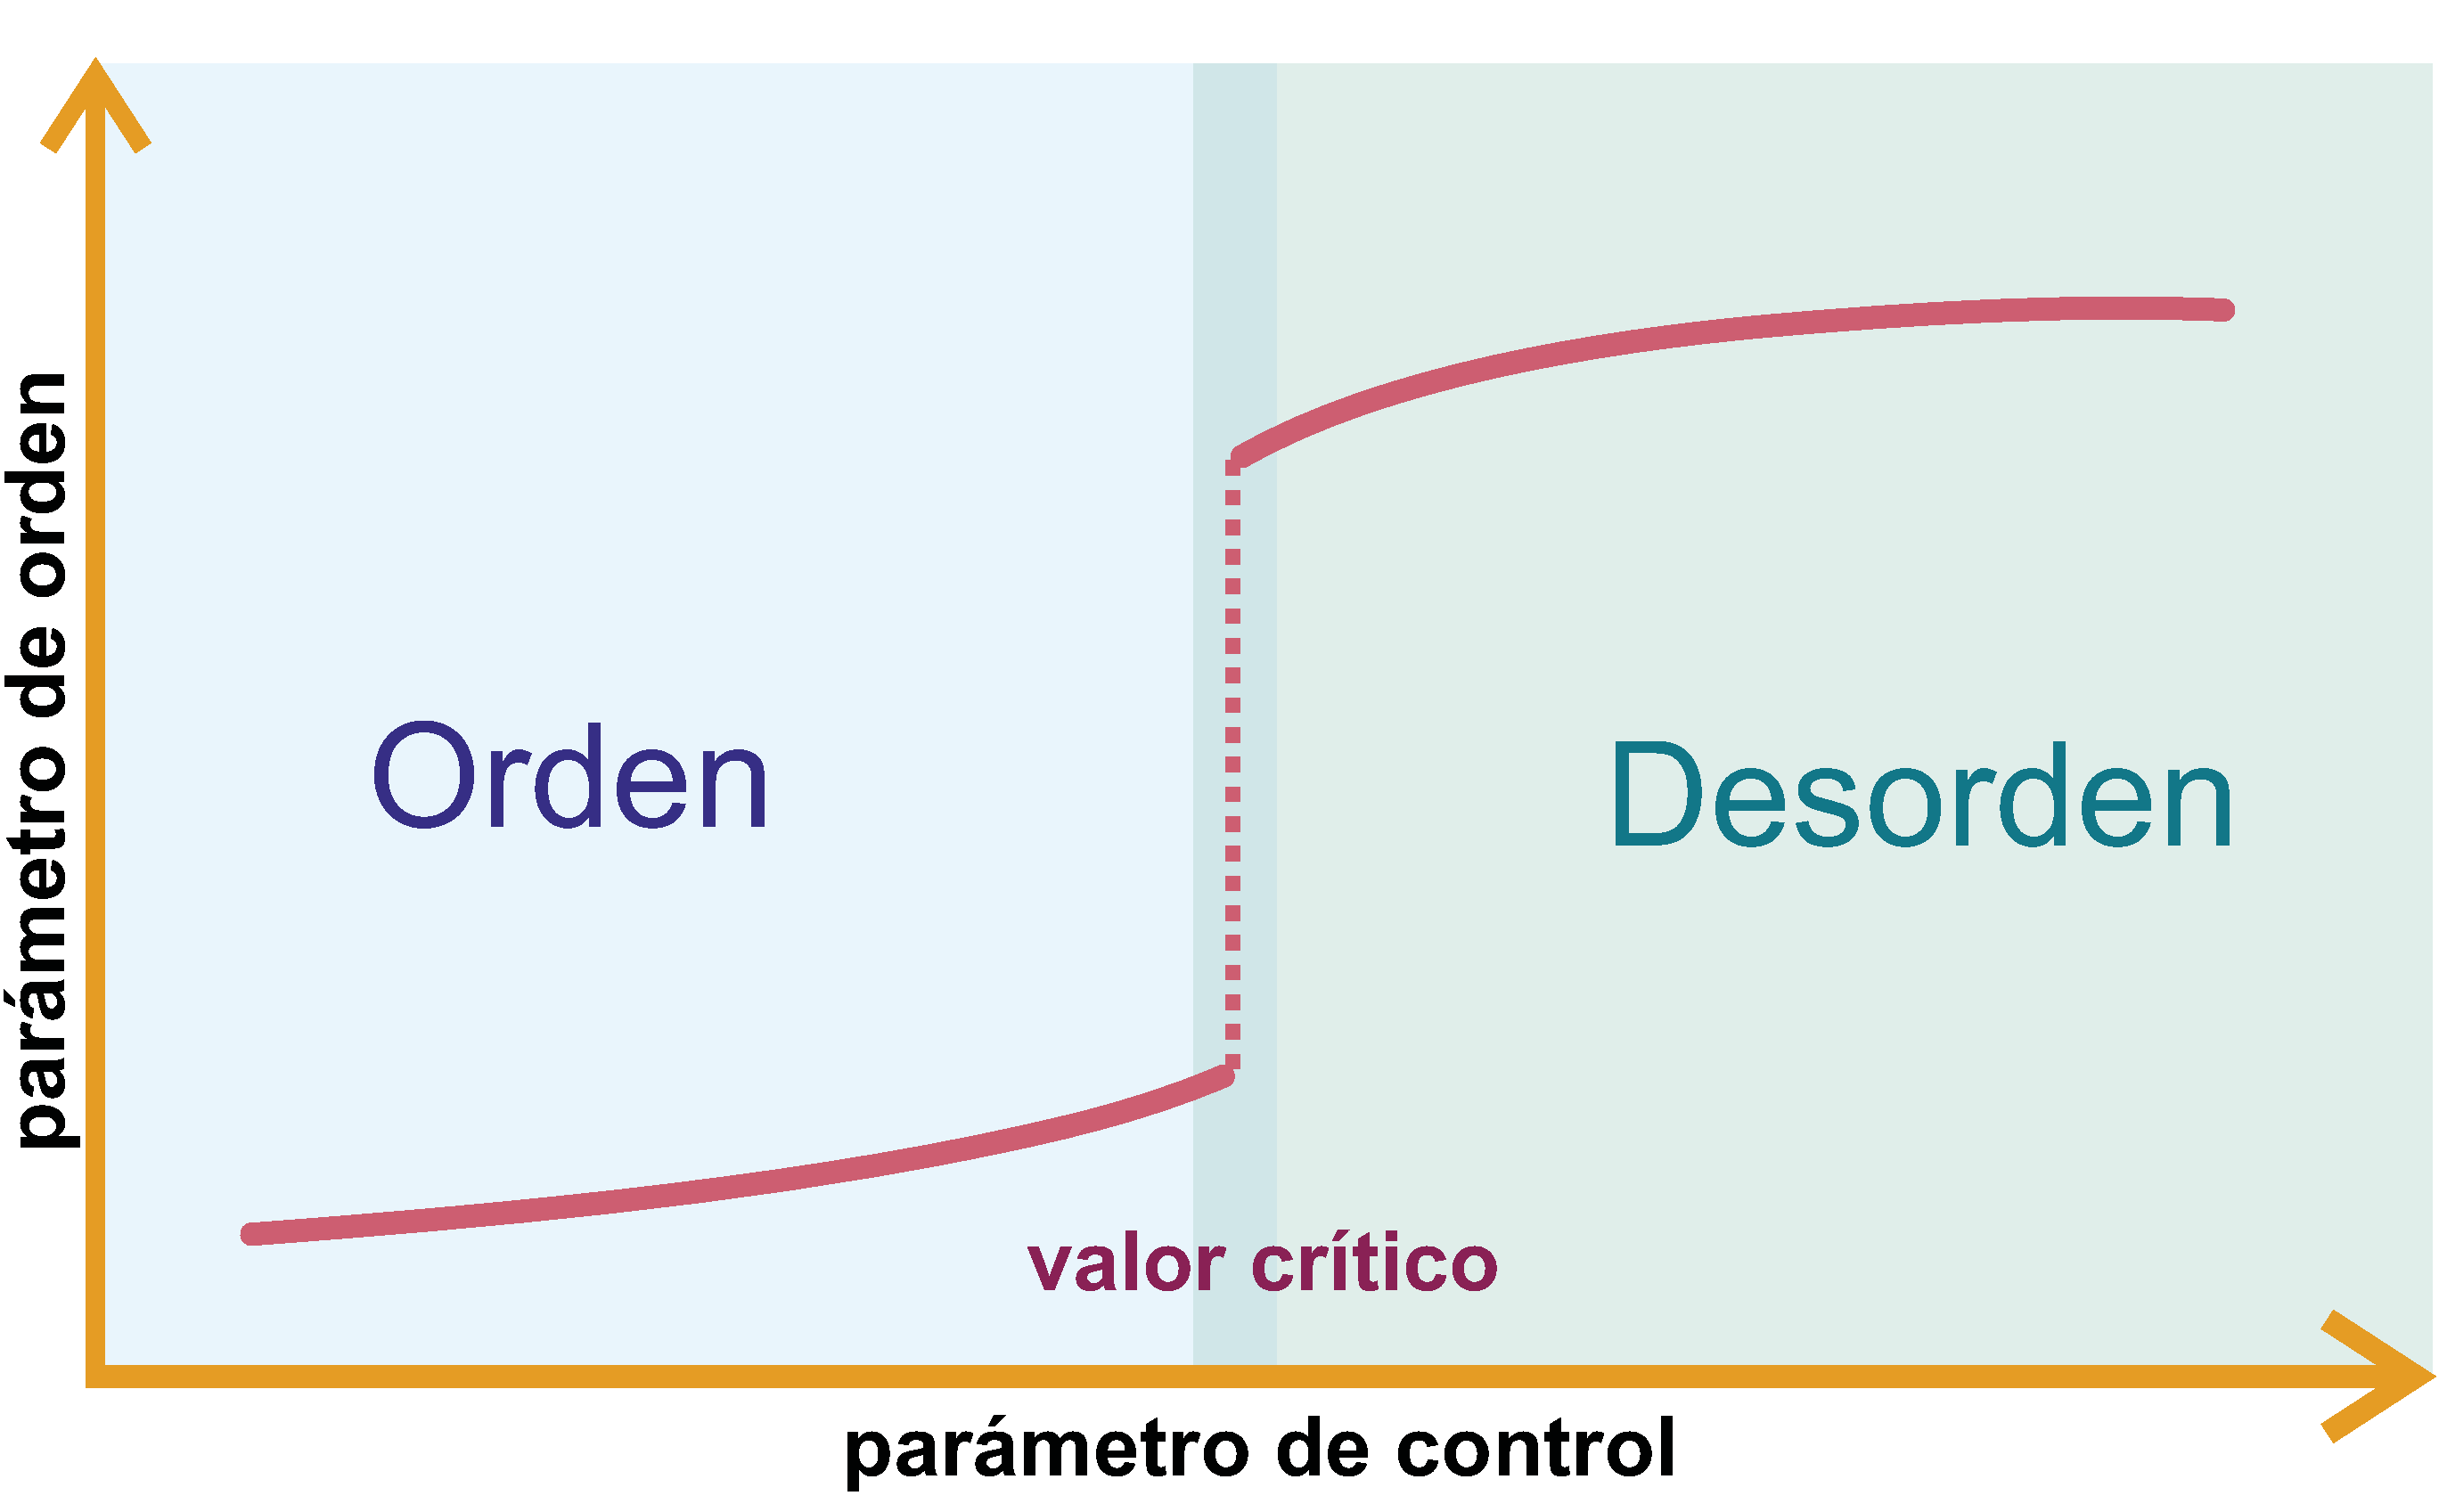
\includegraphics[width=\textwidth]{transiciones_fases_tipo_I.pdf}
		%\caption{transiciones de fase de primer orden}
		\caption{}
		\label{fig:transicionI}
	\end{subfigure}
	\begin{subfigure}[b]{0.45\textwidth}
		\centering
		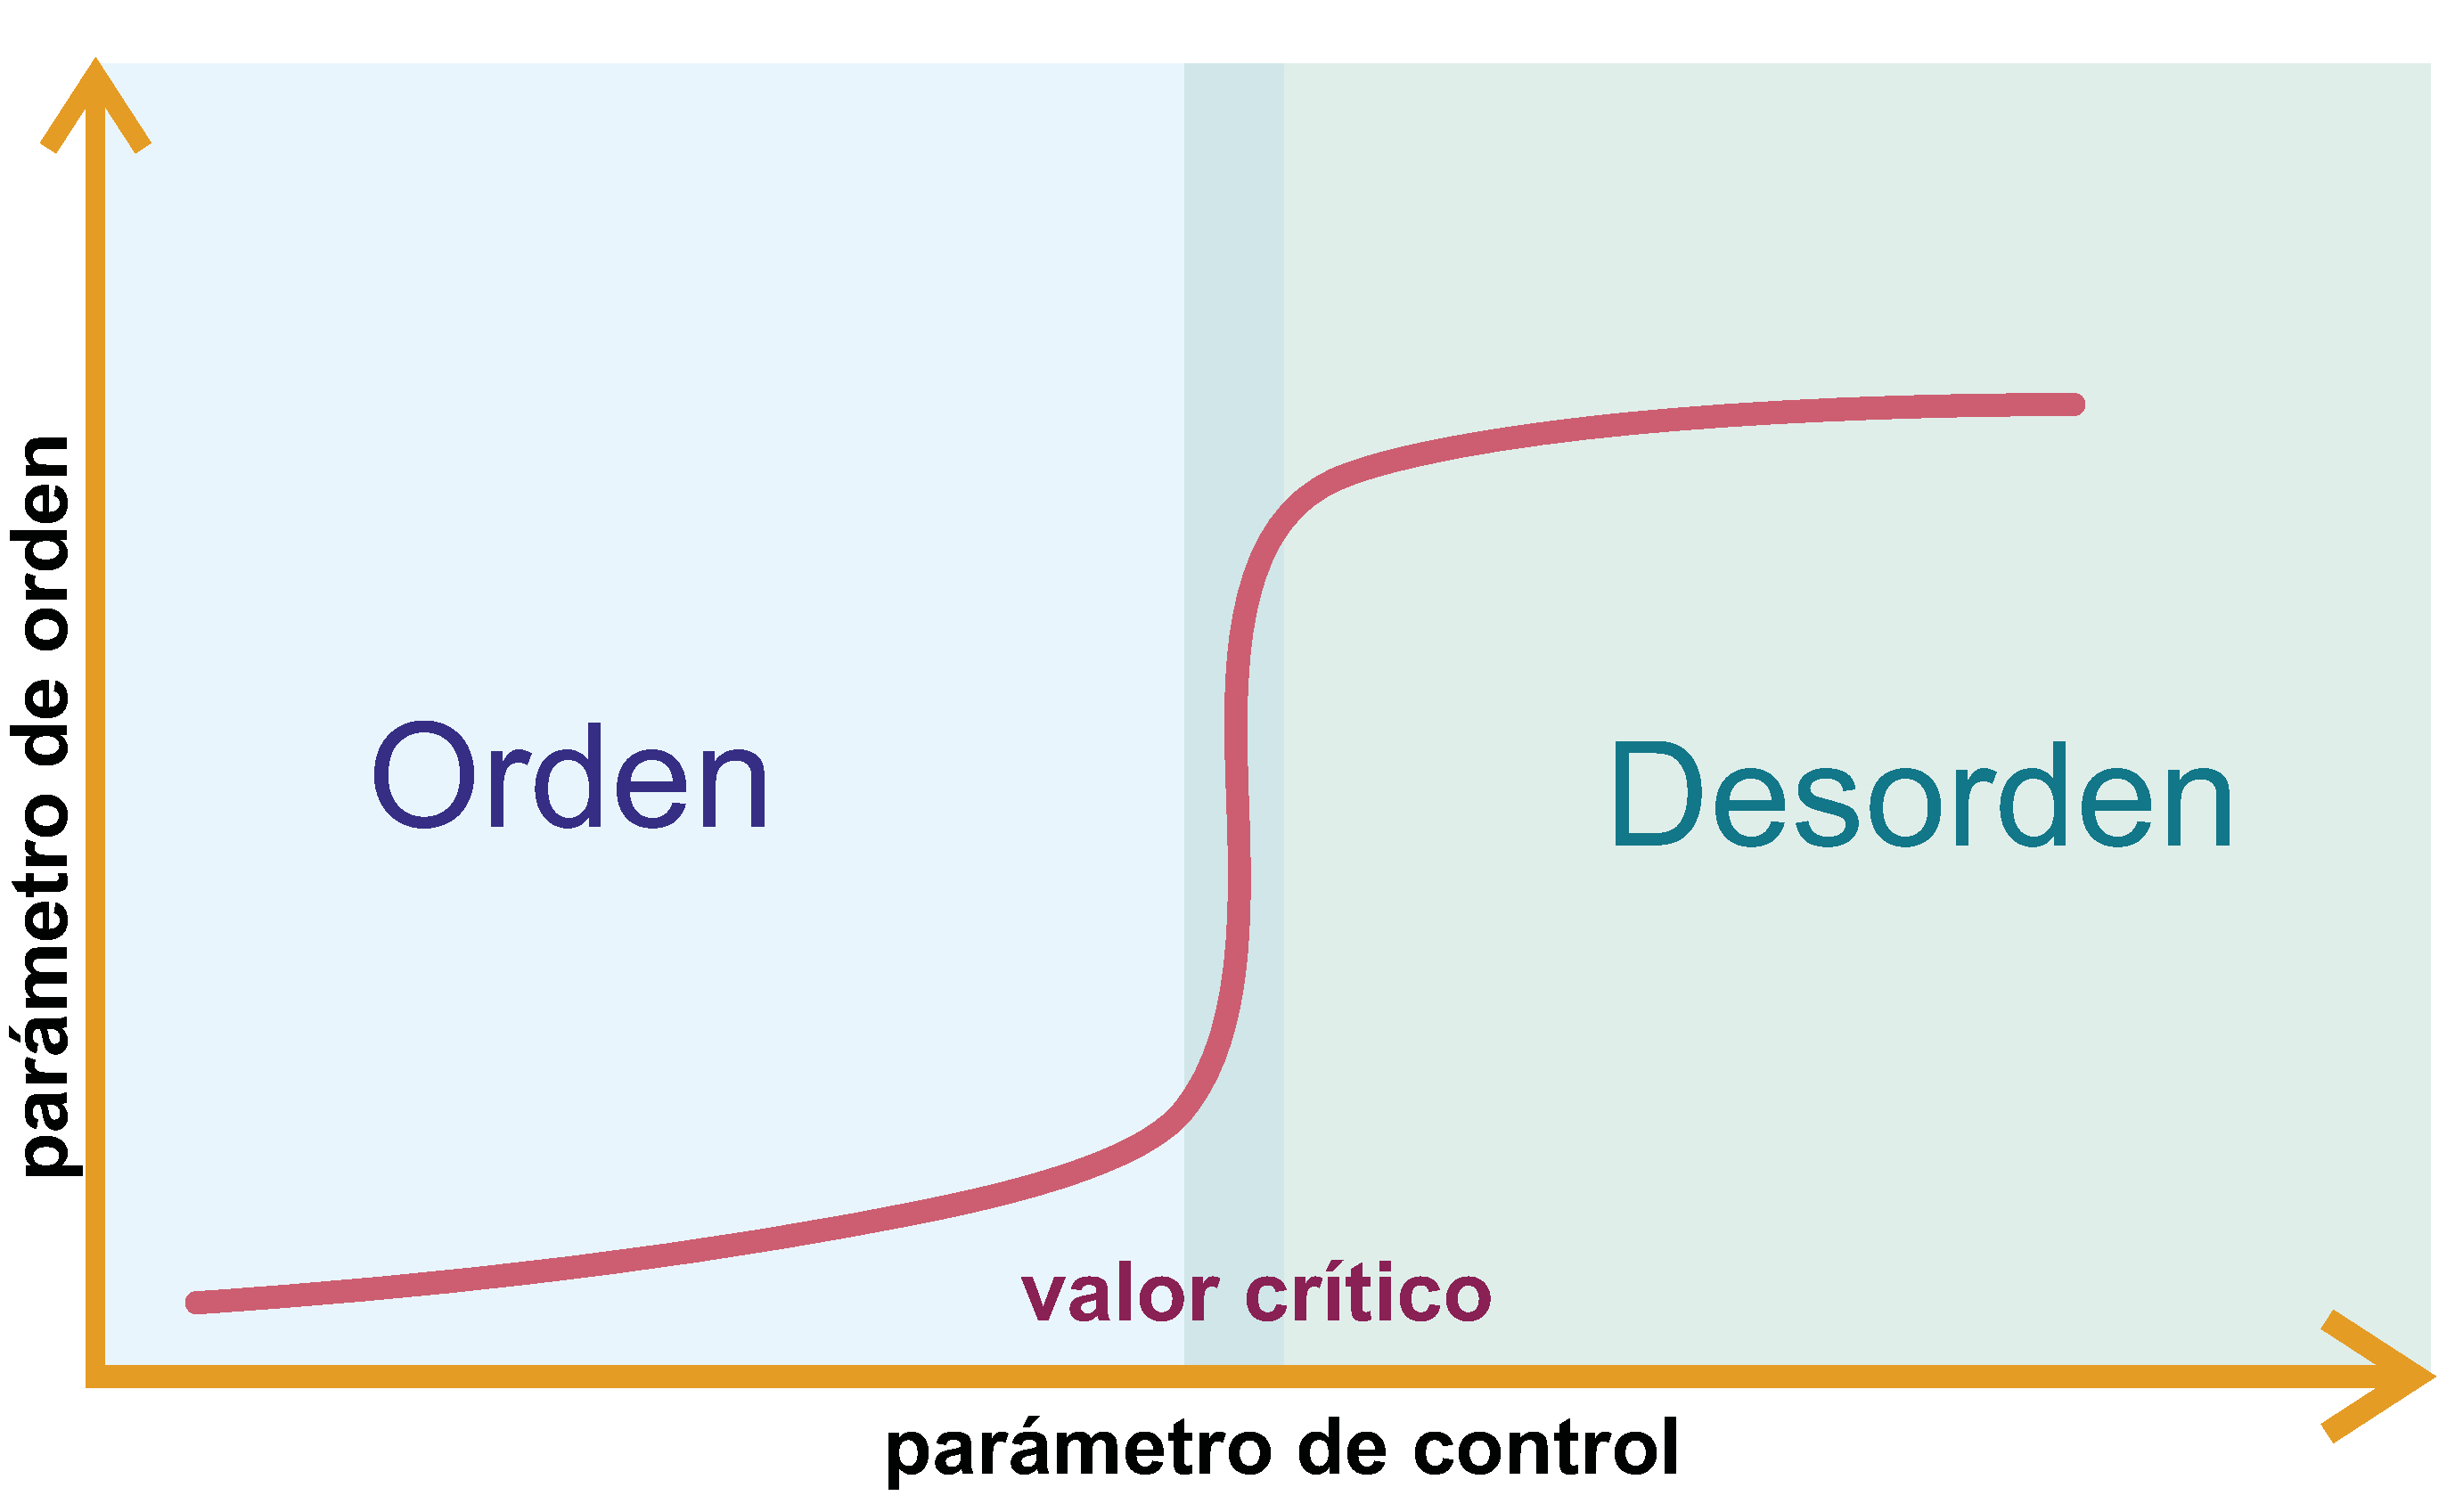
\includegraphics[width=\textwidth]{transiciones_fases_tipo_II.pdf}
		%\caption{transiciones de fase de segundo orden}
		\caption{}
		\label{fig:transicionII}
	\end{subfigure}
	\caption[Representaciones esquemáticas de transiciones de fase de primer y segundo orden.]{Representaciones esquemáticas de transiciones de fase de primer y segundo orden. La figura muestra dos ejemplos de transiciones de fase que ocurren en sistemas termodinámicos. En (a), se ilustra una transición de fase de primer orden, donde el parámetro de orden experimenta un cambio abrupto en su valor crítico del parámetro de control. En contraste, en (b) se muestra una transición de fase de segundo orden, donde el parámetro de orden varía suavemente a medida que cambia el parámetro de control.}
	\label{fig:trancisiones}
\end{figure}


\begin{figure}[h!]
	\centering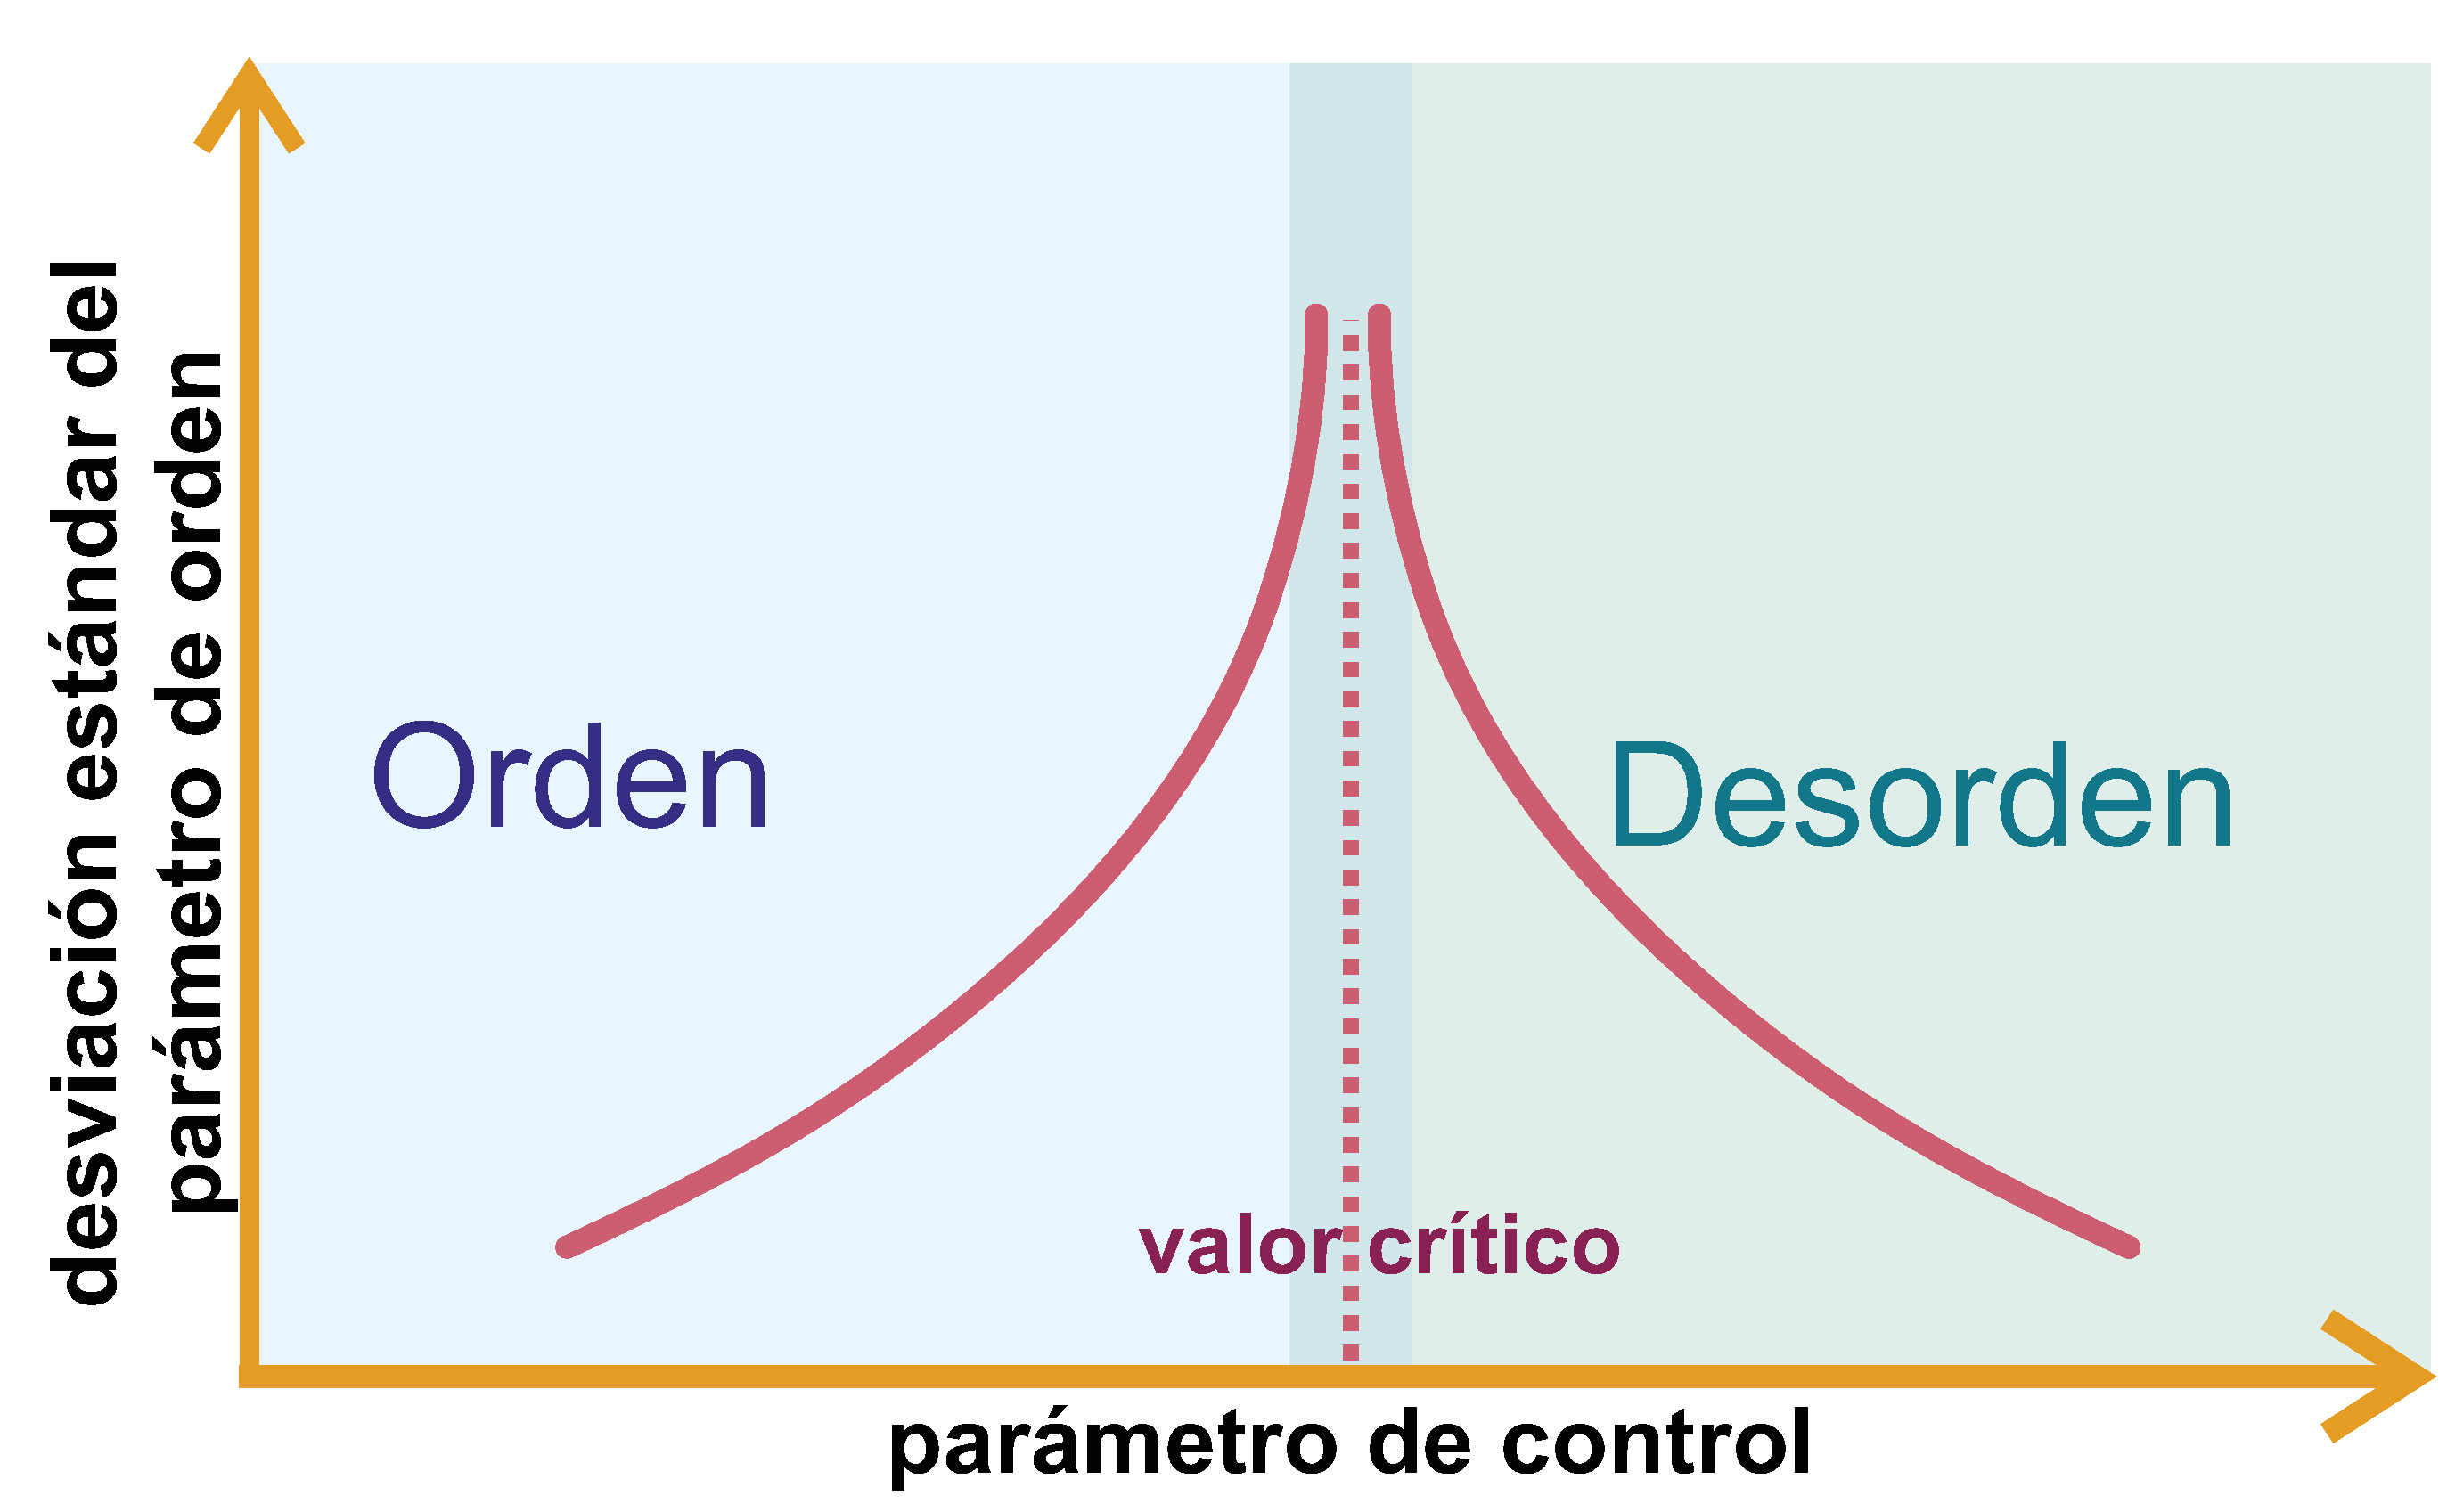
\includegraphics[width=\imsize]{transiciones_fases_tipo_II_divergencia}
	\caption[Desviación estándar del parámetro de orden en transiciones de fase crítica.]{Desviación estándar del parámetro de orden en transiciones de fase crítica. Durante las transiciones de fase crítica, se espera que el parámetro de orden exhiba fluctuaciones significativas. En particular, se observa un aumento en la amplitud de las fluctuaciones en el rango crítico, con la mayor desviación estándar en el valor crítico.} 	\label{fig:divergencia}
\end{figure}


Si un sistema exhibe una transición de fase continua, entonces puede existir en un punto crítico que se encuentra exactamente en la frontera entre dos fases distintas. Este estado límite, conocido como estado crítico, se caracteriza por la presencia de fluctuaciones importantes en el valor del parámetro de orden en el rango crítico, lo cual refleja la pérdida de simetría del sistema que ocurre durante las transiciones de fase. Por consiguiente, se considera que los estados críticos se encuentran en la frontera del caos. Las transiciones de fase críticas son especialmente interesantes debido al comportamiento crítico que se manifiesta en las grandes fluctuaciones del parámetro de orden, las cuales exhiben escalamiento de ley de potencia (Figura 1C).



\subsection{Transiciones de fase en biología}


El principio de universalidad es un concepto ampliamente aceptado en la física que establece que las características relevantes de los fenómenos a gran escala son altamente insensibles a los detalles específicos del modelo y se comparten entre sistemas aparentemente distintos. Siguiendo este principio, se ha propuesto una hipótesis controvertida, pero ampliamente investigada, según la cual algunos sistemas biológicos pueden obtener beneficios funcionales significativos al operar cerca del punto crítico de una transición de fase \cite{munoz_colloquium_2018,hidalgo_information-based_2014,kauffman_origins_1993,bak_how_1996,chialvo_brain_2008,chialvo_emergent_2010,plenz_critical_2013,niebur_criticality_2014,shew_functional_2013,cocchi_criticality_2017,zimmern_why_2020}. En particular, estos sistemas operarían en el límite entre una fase activa o caótica, en la que las fluctuaciones son amplificadas y la información se corrompe, y una fase inactiva u ordenada, en la que las fluctuaciones se amortiguan rápidamente y se reduce la capacidad de respuesta y adaptación. Se han identificado varios ejemplos de tales transiciones, como se resume en el \cref{table:transiciones_biologicas}.

% primer estilo 
%row{odd} = {bg=azure8},
%row{1} = {bg=azure3, fg=white, font=\sffamily},

% segundo estilo 

%row{odd} = {bg=red8},
%row{even} = {bg=red9},
%row{1} = {bg=red3, fg=white, font=\sffamily}

% tercer estilo 

%row{odd} = {bg=gray8},
%row{even} = {bg=gray9},
%row{1} = {bg=red3, fg=white, font=\sffamily},

%otra 

%row{odd} = {bg=teal9},
%row{1} = {bg=teal3, fg=white, font=\sffamily},


\begin{table}[h!]
	\centering
		\caption[Ejemplos seleccionados de transiciones de fase en biología.]{ Ejemplos seleccionados de transiciones de fase en biología, adaptado de Heffern et al\protect{\cite{heffern_phase_2021}}.}
\begin{tblr}{colspec={X[2,l]X[2,l]X[2,l]X[l]},
row{odd} = {bg=gray8},
row{even} = {bg=gray9},
row{1} = {bg=red3, fg=white, font=\sffamily},
}
	sistema	& parámetro de control	  &   parámetro de orden	& referencias seleccionadas\\
	  
	
	Fusión de la membrana plasmática	 & Temperatura	  &  Fluidez &    \cite{de_kruyff_effect_1972} \\
	

	Sincronización neuronal	 &   Fuerza sináptica; relación de excitación a inhibición	 &  Sincronización de tasas de disparo	 &    \cite{adhikari_time-delay-induced_2011,baumgarten_critical_2019}\\
	
	{Agrupamiento/enjambre}	 & Densidad; ruido en la percepción del comportamiento de los vecinos	  & Alineación de patrones de vuelo	  &   \cite{cavagna_scale-free_2010,bahar_flocking_2018,attanasi_finite-size_2014}  \\
	
	Rigidez de actina	 &   Densidad	 &   Rigidez &   \cite{gurmessa_triggered_2019,hussain_spatiotemporal_2013}  \\
	
Colapso de la población microbiana	 	&  Nivel de estrés	 & Crecimiento  &  \cite{mensonides_metabolic_2002,ordway_phase_2020}  \\
	
	Evolución cultural	 &  Cambios en el \gls{fitness} acompañado de \gls{epistasis} entre rasgos culturales	 &  Paradigma cultural	 & \cite{pascual_epistasis_2020}   \\ 
	
	
Rasgos del fitoplancton	 	& Condiciones de luz	  &   Contenido de clorofila	&  \cite{held_second-order_2020}  \\
	
	Colapso de la población de megafauna	 &   Variado& Tamaño de la poblacion	  &  \cite{hein_population_2019,lauerburg_socio-ecological_2020,heinze_quiet_2021}  \\ 
	
	Percolación de rigidez en embriogénesis de pez cebra	 &  Conectividad celular dependiente de la adhesión	 & Viscosidad del tejido, tamaño del grupo	  &  \cite{petridou_rigidity_2021}   \\
	
	\end{tblr}
	\label{table:transiciones_biologicas}
\end{table}

Existen varios experimentos que respaldan esta hipótesis. Algunos de estos ejemplos incluyen las transiciones de fase de sincronización en osciladores biológicos colectivos, como los relojes circadianos \cite{garcia-ojalvo_modeling_2004}; las transiciones de percolación de fibras en tejidos conectivos, como el colágeno \cite{forgacs_phase_1991,newman_phase_2004,alvarado_molecular_2013}; la transición de fase de fusión en hebras de ADN \cite{magee_jr_theory_1963,li_phase_2006}; las transiciones entre diferentes regímenes dinámicos, como las oscilaciones y los estallidos, en redes neuronales \cite{kelso_phase_1984,freeman_metastability_2005,rabinovich_dynamical_2006,werner_metastability_2007,adamatzky_chaos_2013,haken_principles_1996}; los patrones de expresión génica \cite{tsuchiya_self-organizing_2016};  el agrupamiento bacteriano \cite{larkin_signal_2018,ordway_phase_2020}  y la formación de colonias de C. elegans \cite{chen_c_2021}. Para obtener una revisión más completa de las aplicaciones de las transiciones de fase a problemas biológicos, se recomienda consultar la obra de Heffern et al \cite{heffern_phase_2021}.



\section{Hipótesis de la criticidad neuronal}
En línea con lo anteriormente expuesto, la hipótesis de la criticidad neuronal sostiene que el cerebro de los organismos puede estar en un estado crítico en el límite entre diferentes tipos de dinámicas \cite{hesse_self-organized_2014}.  De manera similar a lo que ocurre en los sistemas biológicos, se ha argumentado que la criticidad proporciona a los sistemas neuronales un equilibrio óptimo entre robustez frente a las perturbaciones y flexibilidad para adaptarse a condiciones cambiantes, así como para conferirles capacidades computacionales óptimas \cite{legenstein_edge_2007,tagliazucchi_signatures_2017}, amplios repertorios dinámicos \cite{shew_neuronal_2009}, gran estabilidad de la red \cite{bertschinger_real-time_2004}, transmisión y almacenamiento óptimo de la información \cite{plenz_organizing_2007,beggs_criticality_2007,haldeman_critical_2005,lombardi_balance_2012,vazquez-rodriguez_stochastic_2017}, máxima sensibilidad a los estímulos \cite{kinouchi_optimal_2006,liu_plasticity_2015}  y un comportamiento global coordinado \cite{schneidman_weak_2006,beggs_neuronal_2003}.

Numerosos modelos específicos, como redes booleanas \cite{kauffman_emergent_1984,derrida_random_1986}, máquinas de estado líquido \cite{langton_computation_1990}, redes neuronales y redes de filtración de nanopartículas de plata \cite{carstens_brain-like_2022} , han verificado esta hipótesis (ver también Haykin et al \cite{haykin_what_2007} para una revisión). 

Experimentalmente, se ha evidenciado que los sistemas neuronales parecen mostrar características de los sistemas en estado crítico, lo que sugiere que la hipótesis de la criticidad neuronal podría ser una explicación plausible para la dinámica del cerebro. Estos estudios incluyen:

\begin{itemize}
\item Invariancia de escala de las avalanchas neuronales \cite{fontenele_criticality_2019,beggs_neuronal_2003,beggs_neuronal_2004}  reportadas en diversas especies \cite{hahn_neuronal_2010,petermann_spontaneous_2009,shriki_neuronal_2013}, a través de diferentes técnicas de imagen \cite{tagliazucchi_criticality_2012} y señales electrofisiológicas \cite{linkenkaer-hansen_long-range_2001}. Al igual que en los sistemas biológicos, se ha encontrado que los sistemas neuronales exhiben una dinámica que es independiente de la escala temporal y espacial, lo que sugiere que los procesos neuronales son más similares a los procesos de los sistemas complejos en estado crítico que a los procesos aleatorios o regulares.
\item La presencia de correlaciones espacio-temporales de largo alcance en las fluctuaciones de amplitud de las oscilaciones neuronales \cite{expert_self-similar_2010,fraiman_what_2012,kitzbichler_broadband_2009}, incluida la observación de espectros de potencia $1/f$ de señales \acrshort{MEG}/\acrshort{EEG} registradas simultáneamente \cite{linkenkaer-hansen_long-range_2001}, resonancia magnética funcional  \cite{kitzbichler_broadband_2009} y respuestas cognitivas  \cite{van_orden_human_2005,shew_adaptation_2015}. Estas correlaciones sugieren que los sistemas neuronales exhiben una dinámica compleja y a largo plazo, lo que es consistente con la dinámica en estado crítico.
\item El aumento de la longitud de correlación con el tamaño del sistema \cite{fraiman_what_2012,ribeiro_trial-by-trial_2022,haimovici_brain_2013}. Al igual que en los sistemas biológicos, los sistemas neuronales parecen ser más estables y tener una dinámica más compleja a medida que aumenta el número de componentes.
\end{itemize}




\subsection{Mecanismos homeostáticos de mantenimiento  del estado Crítico}

Es posible conjeturar que la criticidad emerge en los sistemas vivos como resultado de procesos adaptativos y evolutivos que sirven como una plantilla para una mayor complejidad. Esta hipótesis propone que la criticidad podría ser una estrategia organizativa común en biología derivada de la física de las transiciones de fase. Sin embargo, aún hay muchas preguntas sin respuesta sobre la hipótesis de la criticidad.

Una de las principales preguntas es cómo un sistema complejo como el cerebro puede permanecer sintonizado en un estado crítico. Es importante tener en cuenta que la teoría de las transiciones de fase normalmente considera sistemas infinitos, mientras que en sistemas grandes pero finitos, las transiciones de fase se suavizan en un pequeño rango de parámetros. En lugar del punto crítico singular, encontramos una pequeña región que no es técnicamente crítica, pero que aún conserva muchas propiedades de criticidad \cite{moretti_griffiths_2013}. Sin embargo, incluso permanecer en esta región \textquote{crítica}  debería requerir mecanismos que resintonicen activamente el cerebro. La idea general de sistemas que se ajustan a estados críticos a través de procesos descentralizados activos se conoce como criticidad autoorganizada (\gls{soc}, por sus siglas en inglés) \cite{bak_how_1996,christensen_evolution_1998,bornholdt_topological_2000,bornholdt_self-organized_2003}.

El término \gls{soc}  describe las propiedades de los sistemas fuera del equilibrio para alcanzar un estado estacionario caracterizado por correlaciones de largo alcance, que se asemejan a las transiciones de fase de segundo orden cerca del equilibrio. En tales casos, el sistema desarrolla una respuesta multiescala que gradualmente alcanza un estado metaestable con correlaciones espaciales y temporales de largo alcance sin un parámetro de ajuste obvio o una transición de fase (dinámica). Por lo tanto, los estados del  \gls{soc} aparecen como un atractor de la dinámica no lineal en un sistema abierto repetidamente impulsado por fuerzas externas (o endógenas) \cite{tadic_self-organised_2021,gross_adaptive_2007}. 

Sin embargo, los sistemas nerviosos son sistemas no conservativos en contraste con los sistemas \gls{soc}  canónicos como los modelos de pilas de arena \cite{jensen_self-organized_1998,pruessner_self-organised_2012}. Para modelar tales sistemas, se utilizan redes no conservativas de elementos representados por autómatas celulares, mapas de tiempo discretos o ecuaciones diferenciales. Dichos modelos tienen características distintas de los sistemas conservadores. Una gran parte de ellos, en particular las redes neuronales, muestran \gls{SOqC} \cite{bonachela_self-organization_2009,bonachela_self-organization_2010,buendia_feedback_2020} o criticidad débil \cite{palmieri_emergence_2018,palmieri_forest_2020}. Con el tiempo, varios autores propusieron diferentes mecanismos biológicos que podrían eliminar el ajuste fino y convertir a la región crítica en un atractor autoorganizado \cite{kinouchi_mechanisms_2020,zeraati_self-organization_2021,meisel_adaptive_2009,droste_analytical_2013,tetzlaff_self-organized_2010,meisel_failure_2012,rocha_homeostatic_2018,plenz_self-organized_2021,levina_phase_2009,ma_cortical_2019}. La criticidad obtenida no es perfecta, pero es suficiente para dar cuenta de los datos experimentales. Además, los mecanismos (principalmente basados en sinapsis dinámicas, pero también en ganancias neuronales dinámicas, regulación homeostática de la inhibición y umbrales de activación adaptativos) son biológicamente plausibles y deben considerarse como un tema de investigación por derecho propio.


\section{Trastornos cerebrales y alteraciones de la criticidad}


En las anteriores secciones se ha examinado la relación de la criticidad con un comportamiento óptimo de la dinámica cerebral y los mecanismos que la organizan y mantienen. Se ha planteado la hipótesis de que las propiedades dinámicas que caracterizan un estado crítico pueden verse como un marcador importante del bienestar cerebral. En este sentido, las desviaciones de la criticidad pueden ser sintomáticas o causales de ciertas patologías, lo que allana el camino para nuevos diagnósticos y tratamientos.

A pesar del creciente interés en la criticidad biológica en las últimas dos décadas, ha habido una escasez de estudios experimentales y clínicos que conecten la criticidad con las perturbaciones. Debido a que la criticidad representa un estado óptimo para el cerebro, se esperaría que la salida del estado crítico suponga una interrupción en sí misma \cite{heiney_criticality_2021}. Sin embargo, en la práctica, las interrupciones en la dinámica de la red probablemente sean más complicadas que una transición fuera de la criticidad, ya que dichas transiciones pueden ser parte de una actividad saludable.

Es importante destacar que existen aplicaciones clínicas de estos hallazgos en varios trastornos neurológicos, como la epilepsia \cite{osorio_epileptic_2010,witton_rogue_2019,kramer_human_2012,moosavi_criticality_2023,meisel_antiepileptic_2020}, las enfermedades neurodegenerativas como la enfermedad de Alzheimer \cite{stam_disturbed_2005,montez_altered_2009,vysata_change_2014} y la enfermedad de Parkinson \cite{hohlefeld_long-range_2012,herrojo_ruiz_long-range_2014,west_parkinsonian_2016}, derrames cerebrales \cite{rocha_recovery_2022}, así como otros dominios clínicamente relevantes, como la anestesia \cite{alonso_dynamical_2014,thiery_long-range_2018,liu_scale-free_2014}, la medicina del sueño \cite{bocaccio_avalanche-like_2019} (incluyendo el insomnio \cite{meisel_decline_2017,colombo_more_2016}, la apnea del sueño \cite{lo_asymmetry_2013} y la narcolepsia), neurodesarrollo \cite{padilla_breakdown_2020,smit_scale-free_2011,mares_age-dependent_2013}, la cognición, atención, aprendizaje y autismo \cite{ezaki_closer_2020,jia_attenuation_2018,ouyang_decomposing_2020,tinker_power_2014,dimitriadis_altered_2013}, efectos psicológicos del neurofeedback y los psicodélicos \cite{zhigalov_modulation_2016,tagliazucchi_enhanced_2014}, las afecciones psiquiátricas comunes como la depresión \cite{gartner_aberrant_2017}, la esquizofrenia \cite{moran_long-range_2019}, la ansiedad \cite{tolkunov_power_2010} y el trastorno de estrés postraumático \cite{ros_tuning_2014}.  Se dispone de una revisión muy completa de estos temas en el artículo escrito por Vincent Zimmern \cite{zimmern_why_2020}.

No obstante, a pesar de los avances en la investigación, todavía no se ha incorporado la criticidad en la práctica clínica habitual. Esto se debe en parte a la falta de estudios experimentales y clínicos que conecten la criticidad con las perturbaciones, y también a la necesidad de formación de equipos multidisciplinarios en los que los físicos, matemáticos, científicos de datos y médicos colaboren para responder mejor a una pregunta clínica a través de la lente de la criticidad.

En este contexto, se espera que el futuro de la criticidad en el ámbito clínico dependa en gran medida de la formación de estos equipos multidisciplinarios y de la aplicación de técnicas de análisis cuantitativo de electroencefalografía (\gls{EEG}), \glossary{MEG} y resonancia magnética funcional (\gls{fMRI}), entre otras. De esta forma, podrían desarrollarse nuevas herramientas diagnósticas y terapéuticas que permitan una mejor comprensión y tratamiento de diversas enfermedades neurológicas y psiquiátricas.



\section{Métricas experimentales de criticidad}


En las secciones anteriores se ha presentado la hipótesis de criticidad y su relevancia en los sistemas biológicos, así como sus limitaciones y aplicaciones. En esta sección, se aborda la detección de las transiciones de fase y la dinámica crítica en experimentos y simulaciones.
La construcción de un diagrama de fase es la evidencia más directa de una transición de fase (ver \Cref{fig:trancisiones} ) \cite{dickman_paths_2000}. En este tipo de diagrama, se puede observar la respuesta del parámetro de orden ante las variaciones del parámetro de control, lo que permite detectar la existencia de una transición de fase. Sin embargo, la construcción de dicho diagrama requiere que el parámetro de control sea accesible y controlable en el entorno experimental, lo que puede resultar difícil en sistemas biológicos complejos.

Por ejemplo, la variación de la conectividad cerebral in vivo puede ser difícil de lograr experimentalmente. Debido a estas limitaciones, la mayor parte de la evidencia de la criticidad en sistemas biológicos proviene de la observación de características distintivas en los resultados experimentales. En esta sección, se discuten las características distintivas de la criticidad que se han identificado en la literatura científica y que se utilizan para establecer la presencia de criticidad en sistemas biológicos \cite{hesse_self-organized_2014}. Estas características distintivas son fundamentales para la identificación de la dinámica crítica en sistemas biológicos complejos, especialmente aquellos cuya dinámica interna es imposible o difícil  de modificar.



\subsection{Escalamiento de la ley de potencia}\label{sec:leypotencia_intro}


En el ámbito de la estadística, una variable aleatoria continua $X$ se considera que tiene una distribución de ley de potencia cuando se extrae de una distribución de probabilidad con densidad $	\mathbb{P}\left(x\leq X\leq x+dx\right)=Cx^{-\alpha}dx$. El parámetro $\alpha$ se conoce como el exponente o parámetro de escala, mientras que $C$ es un parámetro de normalización. Por otro lado, una variable aleatoria discreta de ley de potencia tiene una versión discretizada similar de la probabilidad, que se puede expresar como 	$P(X=k)=Ck^{-\alpha}$.

Es importante señalar que en la práctica, son pocos los fenómenos empíricos que obedecen leyes de potencia para todos los valores de $X$. En general, las leyes de potencia se utilizan para caracterizar la cola de la distribución, es decir, la distribución de probabilidad de los valores de $X$ mayores que algún valor $x_{min}$. En estos casos, se dice que la cola de la distribución sigue una ley de potencia. Además, los datos a menudo muestran una distribución de ley de potencia truncada, lo que significa que el comportamiento de ley de potencia solo se observa en un rango limitado, $x_{min}\leq X \leq x_{max}$  \cite{touboul_can_2010}.

Cabe destacar que las leyes de potencia presentan invariancia de escala, lo que las convierte en distribuciones libres de escala. Una función $f(x)$ se considera invariante de escala si $ f(cx)  = \left(cx\right)^{-\alpha}=c^{-\alpha}x^{-\alpha}=c^{-\alpha}f(x)\propto f(x)$, lo que indica que escalar el argumento de la función es equivalente a escalar proporcionalmente la función misma. Además, como $\log(p(x))=\log_{\alpha}\left(ax^{-\alpha}\right) = -\alpha\log(x)+\log(a)$, el histograma de la ley de potencias presenta una relación afín en un gráfico logarítmico (\Cref{fig:leypotencia}).

Debido a esto, las leyes de potencia en datos empíricos se suelen analizar graficando el logaritmo del histograma en función del logaritmo de los valores de la variable aleatoria. Luego, se aplica un algoritmo de mínimos cuadrados para ajustar una línea afín a través de los puntos de datos. Este método se remonta a Pareto en el siglo XIX \cite{arnold_pareto_2008}. Sin embargo, es importante destacar que la inspección visual de un diagrama puede generar falsos positivos. Además, se ha señalado que las pruebas convencionales de bondad de ajuste no son adecuadas para las leyes de potencia \cite{newman_power_2005}.



\begin{figure}[h!]
	\centering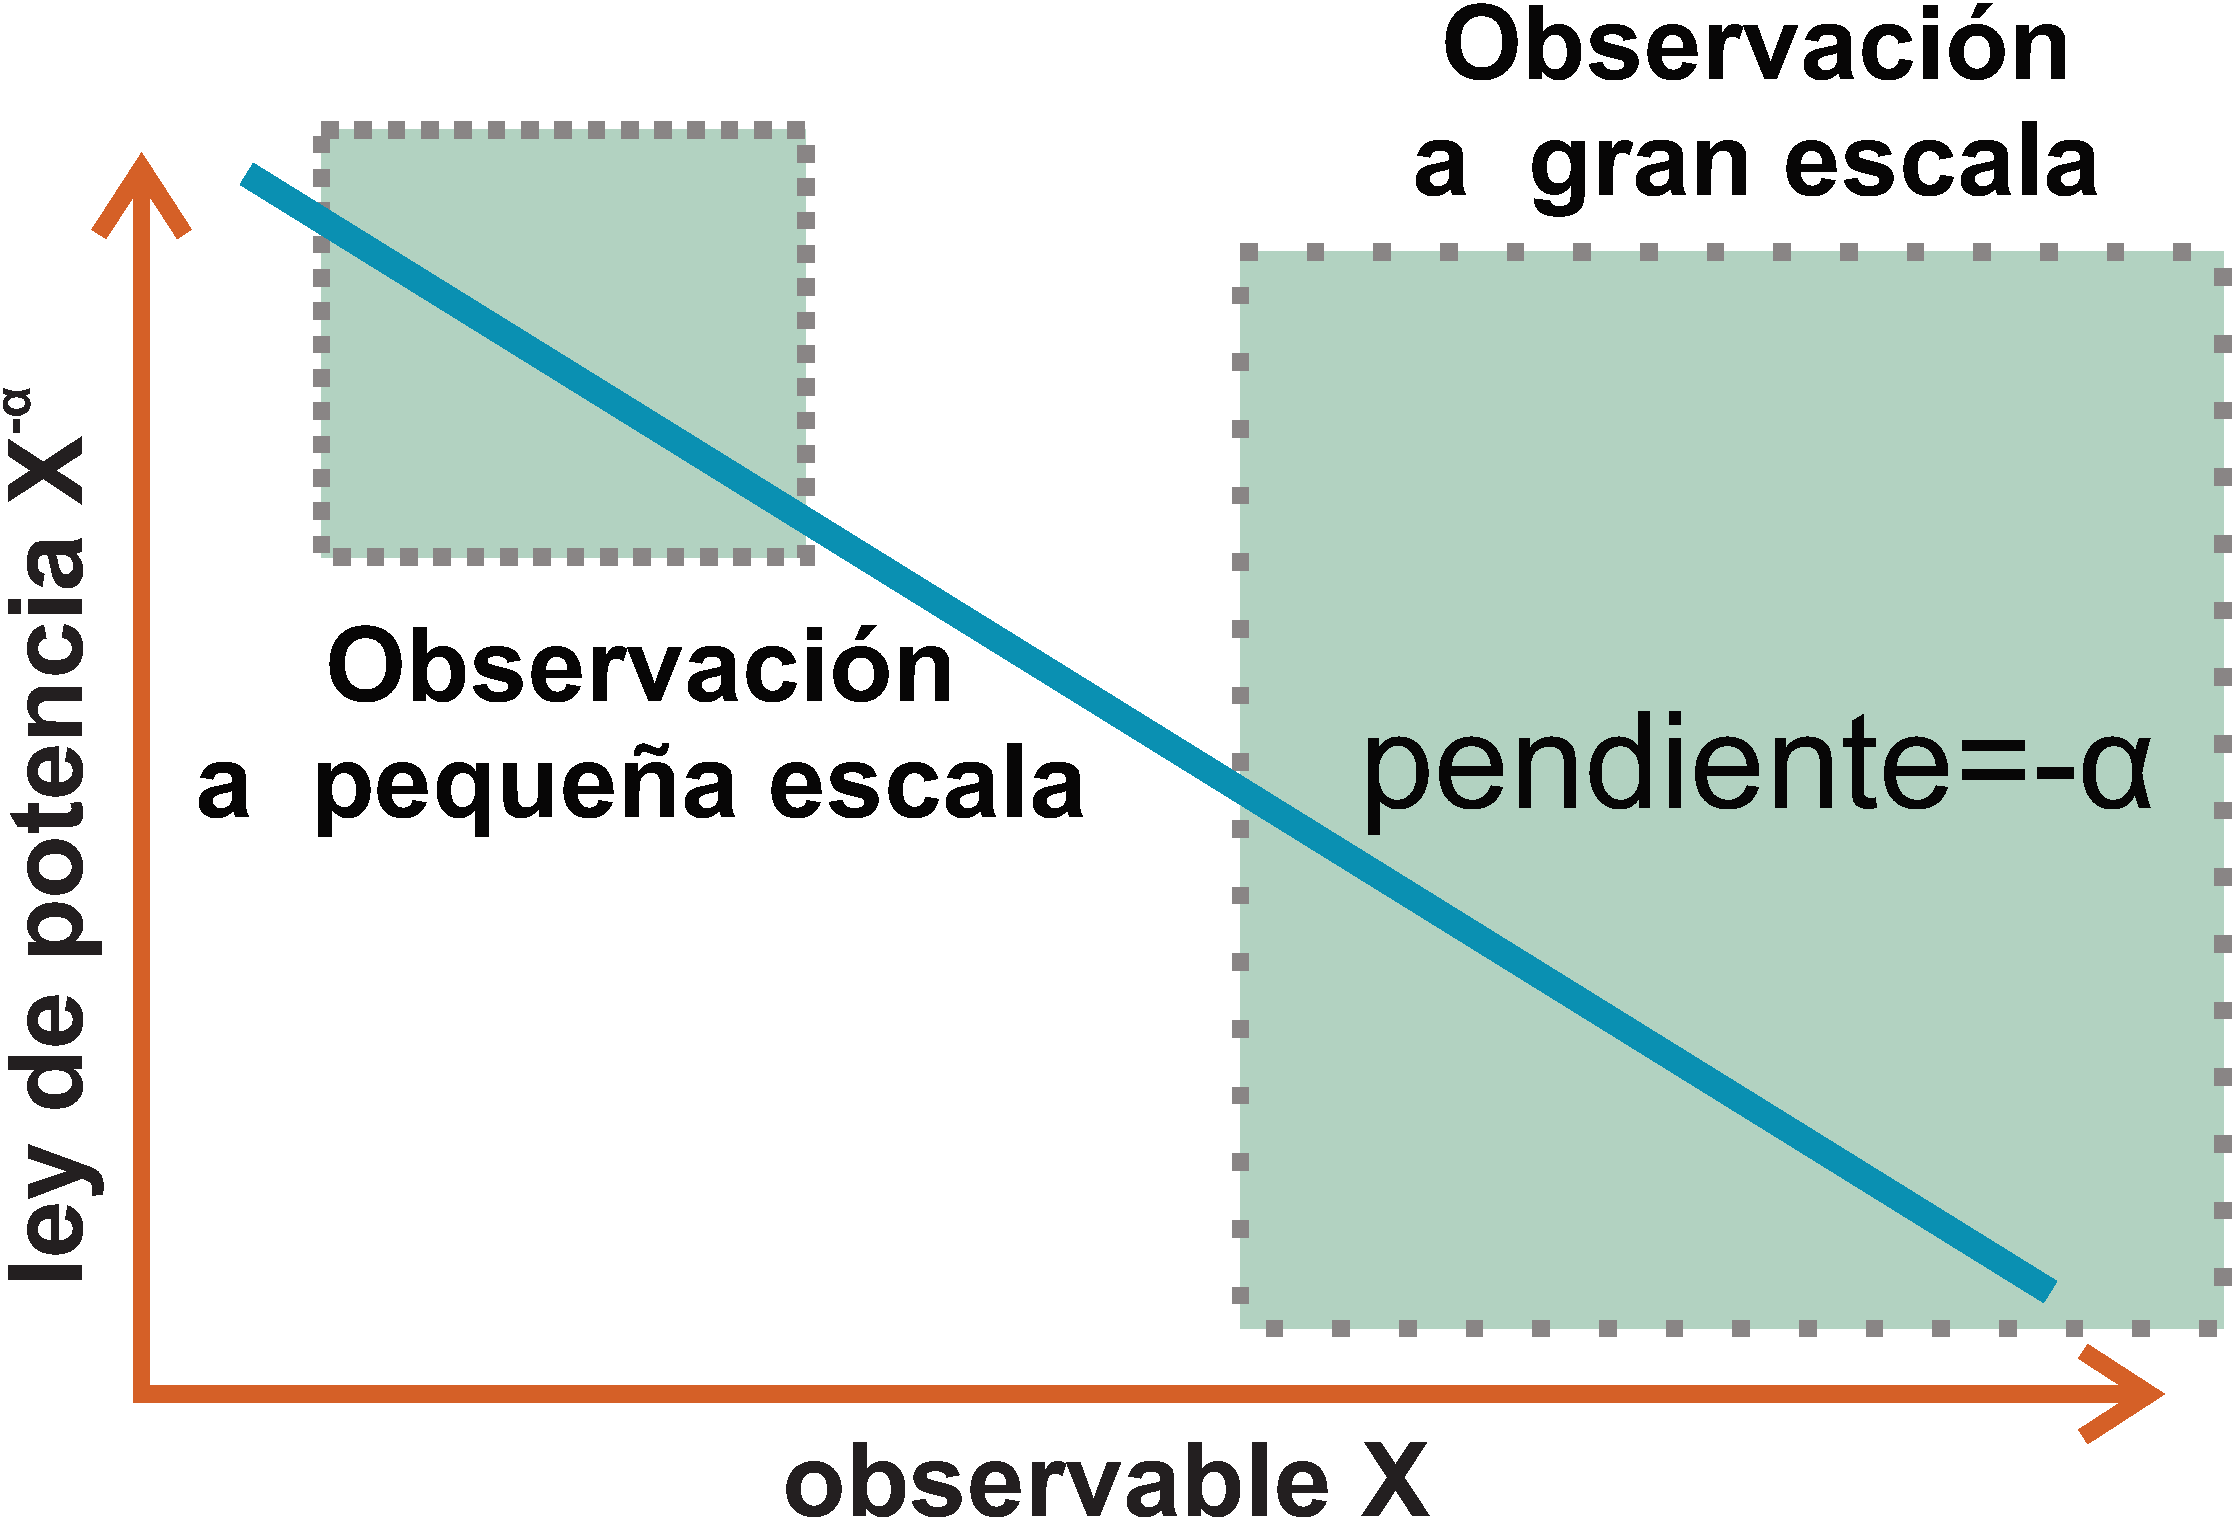
\includegraphics[width=\imsize]{ley_potencia}
	\caption[Representación gráfica de la independencia de escala de las leyes de potencia en una distribución de datos.]{Representación gráfica de la independencia de escala de las leyes de potencia en una distribución de datos, donde se ha utilizado la ley de potencia $f(x) = x^{-\alpha}$  con un exponente crítico de $\alpha=-1.5$ y una escala logarítmica en el eje $x$. La figura muestra que, independientemente del rango o escala utilizada para medir la distribución, se observa una ley de potencia con el mismo exponente crítico.} 	\label{fig:leypotencia}
\end{figure}


La hipótesis de criticidad en experimentos y simulaciones se basa en la presencia de leyes de potencia, que se espera se manifiesten en la mayoría de los sistemas críticos. Sin embargo, la existencia de leyes de potencia por sí sola no es suficiente para probar la criticidad \cite{goldstein_problems_2004,priesemann_can_2018}, ya que estas leyes también pueden ser explicadas por mecanismos no críticos \cite{touboul_can_2010,markovic_power_2014,noauthor_critical_2006,beggs_being_2012}. Por tanto, la identificación de leyes de potencia es un asunto delicado que requiere procedimientos de ajuste avanzados, debido a la dificultad para diferenciarlas de otras distribuciones de colas pesadas.

Las distribuciones de cola pesada son aquellas distribuciones de probabilidad cuyas colas son \textquote{más pesadas} que la distribución exponencial, siendo la gaussiana un subtipo de esta última. Entre los ejemplos de distribuciones de cola pesada se encuentran la distribución de Fisher-Tippett (doble exponencial), la distribución logarítmica normal y la distribución de Weibull, entre otras. Aunque se espera la presencia de leyes de potencia en sistemas críticos, estas distribuciones también pueden presentarse en otros sistemas no críticos. Por ende, para una mejor comprensión de la relevancia de las distribuciones de cola pesada en la neurociencia, se sugiere consultar la obra de Roberts et al  \cite{roberts_heavy_2015}.

Para abordar esta problemática, los investigadores han tenido acceso a metodologías estadísticas más sofisticadas gracias a los trabajos realizados por Clauset et al  \cite{clauset_power-law_2009} y otros estudios posteriores \cite{klaus_statistical_2011,markovic_power_2014}. Estas metodologías permiten distinguir las leyes de potencia de otras distribuciones de colas pesadas y evaluar su presencia en sistemas críticos. Sin embargo, es importante tener en cuenta que las leyes de potencia se truncan en sistemas de tamaño finito \cite{bonachela_self-organization_2010} y pueden verse afectadas por el submuestreo \cite{ribeiro_undersampled_2014}. Por lo tanto, es necesario emplear medidas cuantitativas para evaluar la diferencia entre las distribuciones de probabilidad acumulada experimental y ajustada por ejemplo  a través del parámetro $\kappa$ \cite{shew_neuronal_2009}.



\subsection{Escalamiento de  la ley de potencia de las avalanchas neuronales }

Beggs y Plenz demostraron experimentalmente que el comportamiento espontáneo de las redes corticales in vitro exhibe características consistentes con dinámicas críticas en su estudio histórico sobre avalanchas neuronales en cortes corticales interconectados con arreglos de microelectrodos (\gls{MEA}) \cite{beggs_neuronal_2003} . Una avalancha neuronal es una duración de actividad persistente que se propaga a través de la red y está marcada por períodos de silencio que preceden y siguen al período activo (ver \Cref{fig:avalancha}). En el caso de sistemas in vitro (es decir, cortes o cultivos disociados), la \textquote{actividad } puede referirse a los picos de mayor frecuencia o el \gls{LFP} de menor frecuencia, ya que se han estudiado ambas modalidades.

\begin{figure}[h!]
	\centering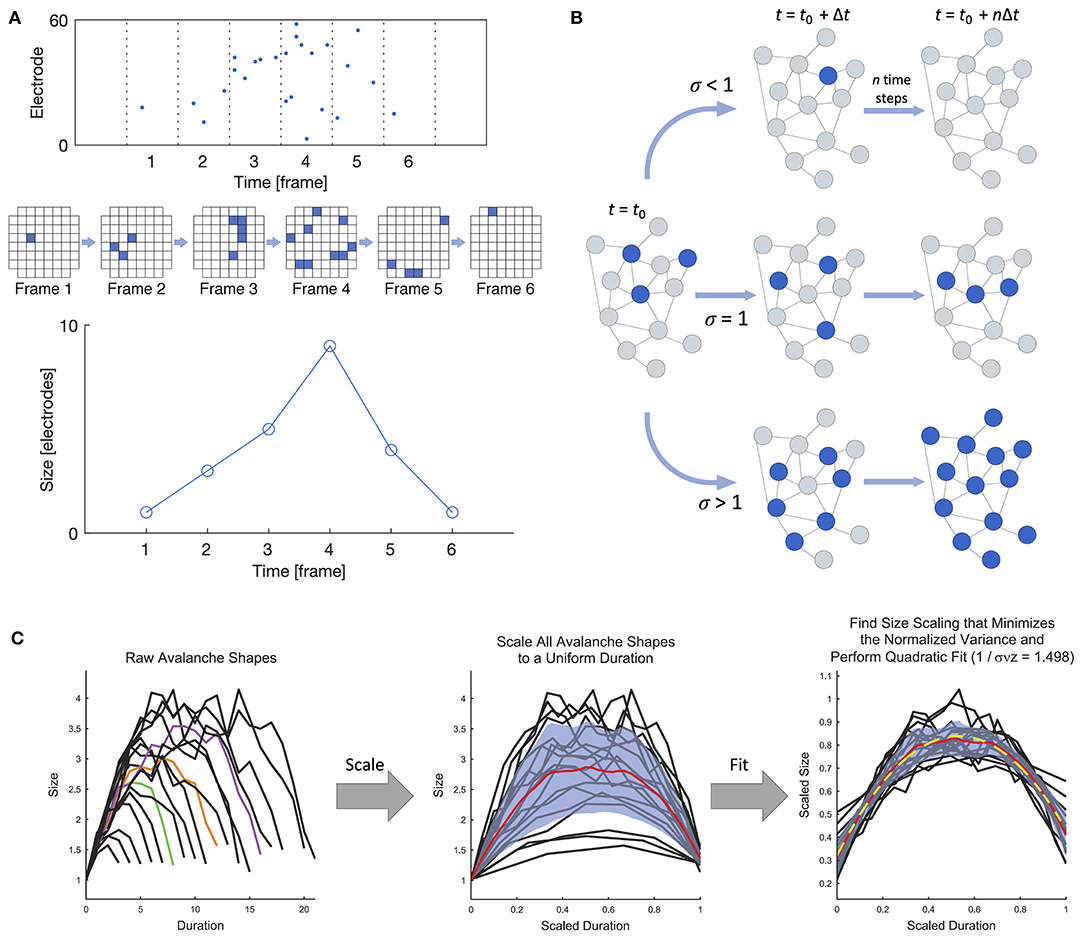
\includegraphics[width=\imsizeL]{fncom-15-611183-g002.jpg}
	\caption[Definición de avalancha neuronal y ejemplos de medidas empíricas de criticidad. ]{Definición de avalancha neuronal y ejemplos de medidas empíricas de criticidad. 
		(a) Se presenta la definición de avalancha neuronal, mostrando en el panel superior un gráfico rasterizado dividido en intervalos de tiempo. La avalancha representada abarca seis fotogramas activos, precedidos y seguidos por fotogramas inactivos. A continuación, se muestra una vista alternativa de la actividad en los seis marcos, en la que cada cuadrado representa un electrodo activo en una cuadrícula de 8x8. El panel inferior exhibe la definición de la forma de avalancha, la cual se obtiene a partir del número de electrodos activos en cada cuadro.
		(b) Se ilustra la relación de ramificación, en la cual los nodos azules representan actividad activa y los grises, inactiva. En una relación de ramificación de 1, la actividad persiste sin sobrecargar el sistema.
		(c) Se observa el colapso de forma en un sistema crítico, donde todas las avalanchas deberían mostrar el mismo perfil de forma temporal media en diferentes escalas de tamaño.
		Esta representación ha sido adaptada de Heiney et al.  \protect{\cite{heiney_criticality_2021}}.} 	\label{fig:avalancha}
\end{figure}


El escalamiento de la ley de potencia del tamaño $S$ y la duración $T$ de las avalanchas neuronales es un sello distintivo de la criticidad en las redes neuronales. Es decir, $P(S) \propto S^{-\alpha}$  y $P(T) \propto T^{-\beta}$, donde $P(\cdot)$  es la función de distribución de probabilidad. El tamaño se define generalmente como el número de electrodos o neuronas activados, y la duración es el número de intervalos de tiempo activos. Los exponentes de la ley de potencia del tamaño y la duración son aproximadamente $\alpha=1.5$ y $\beta= 2.0$, respectivamente, cuando se selecciona el ancho del intervalo de tiempo para que se corresponda con el intervalo promedio entre picos. Sin embargo, la escala de la ley de potencia debe persistir en un rango de resoluciones temporales cercano al orden de magnitud del intervalo promedio entre picos, con el exponente $\alpha$ cambiando sistemáticamente con el tamaño del intervalo de tiempo seleccionado \cite{beggs_neuronal_2003,pasquale_self-organization_2008}. La escala de ley de potencia también debe mantenerse cuando se considera una resolución espacial de grano más grueso, utilizando solo un subconjunto de todos los puntos de registro. Las redes neuronales pueden mostrar varios puntos críticos dinámicos únicos, de los cuales solo uno es la transición de fase que da lugar a las avalanchas neuronales. Por lo tanto, es crucial considerar el contexto más amplio y no limitarse a la transición de fase en sí misma \cite{kanders_avalanche_2017}.







\subsection{Parámetro de ramificación}



En la teoría de los procesos de ramificación \cite{harris_theory_1963} se utiliza una medida común, la relación de ramificación $\sigma$, para evaluar el número de descendientes y ancestros en un sistema. En particular, esta medida establece la proporción entre el número de descendientes y el número de ancestros, en el que la actividad en un electrodo o neurona ancestro precede inmediatamente a la actividad en un electrodo o neurona descendiente \cite{beggs_neuronal_2003}. En un sistema en estado crítico, la relación de ramificación se aproxima a $1$, lo que permite que la actividad fluya a través de la red sin extinguirse ($\sigma < 1$) o saturar toda la red ($\sigma > 1$), tal como se muestra en la \cref{fig:avalancha}. Por tanto, la presencia de una relación de ramificación $\sigma = 1$ en respuesta a una excitación artificial en un sistema lo suficientemente inactivo puede considerarse como una evidencia de criticidad.

No obstante, es importante destacar que, en comparación con otras características, la evidencia proporcionada por una relación de ramificación de uno es relativamente débil. Esto se debe a que dicha relación no implica necesariamente una dinámica crítica, ya que también puede ser observada en estados supercríticos \cite{hesse_self-organized_2014}. Por lo tanto, se requiere de un análisis más riguroso que permita distinguir entre ambos estados.


\subsection{Colapso de forma}


La dinámica de los sistemas críticos se caracteriza por la presencia de avalanchas de actividad, que exhiben una naturaleza autosimilar o fractal. Se espera que la \textquote{forma} de la actividad de la avalancha se comporte como un fractal en dichos sistemas. En un estado crítico, se espera que todas las avalanchas muestren el mismo perfil temporal medio en todas las escalas. El perfil temporal de una avalancha se define como el número de sitios activos en función del tiempo. Para un sistema en estado crítico, los perfiles temporales de todas las avalanchas colapsan en la misma forma de perfil cuando se escala espacio-temporalmente con un exponente de escala$\gamma$ cercano a $2$(\Cref{fig:avalancha}). Esta propiedad se describe por  $ \left\langle S\right\rangle(T) \propto T^{-\gamma}$, donde $\left\langle S\right\rangle(T)$  representa el tamaño promedio de todas las avalanchas de una duración determinada $T$.

Se puede encontrar información detallada sobre el colapso de la forma en la literatura científica, como en Sethna et al \cite{sethna_crackling_2001} y Friedman et al \cite{friedman_universal_2012}. Además, Miller et al \cite{miller_scale-invariant_2019} proporciona una demostración experimental del colapso de la forma en primates no humanos. El coeficiente de criticidad (DCC) de Ma et al \cite{ma_cortical_2019} se relaciona con el concepto de colapso de forma y se calcula a partir de la diferencia entre el exponente de escala $\gamma$, obtenido a partir de datos empíricos mediante regresión lineal, y el valor esperado obtenido a partir del exponente de ley de potencia $\alpha$ de la distribución de tamaños.


\subsection{Submuestreo espacial}

Debido a la naturaleza intrínseca de la observación de los sistemas neuronales, se ve limitada la capacidad de muestrear todos los componentes del sistema. Como consecuencia, se puede obtener únicamente una muestra espacialmente submuestreada del sistema, la cual puede resultar insuficiente para obtener conclusiones precisas acerca de la dinámica subyacente del sistema. Para abordar este problema, se han desarrollado métodos que involucran el escalado del submuestreo espacial \cite{levina_subsampling_2017} y el uso de un estimador invariante de submuestreo \cite{wilting_inferring_2018}. Estos métodos permiten la evaluación precisa de los estados dinámicos de sistemas submuestreados, incluso en situaciones donde el número de componentes muestreados es significativamente menor que el número total de componentes del sistema.



\subsection{Correlación temporal de largo alcance, ralentización crítica y flickering}


En sistemas críticos, la respuesta del sistema a los estímulos externos se maximiza, lo que se conoce como rango dinámico o correlación dinámica. La criticidad del sistema genera retornos geométricos al estado estacionario \cite{hesse_self-organized_2014}, lo que resulta en una correlación temporal de largo alcance \gls{LRTC} o memoria larga. La \gls{LRTC} puede medirse de diversas maneras, siendo los métodos más populares el exponente de Hurst, a través de varios estimadores, y   \gls{DFA}  \cite{hardstone_detrended_2012}. Este último produce un exponente de escala durante un período de tiempo determinado. Un exponente de escala entre $0.5$ y $1$, con un buen ajuste, indica que la serie de tiempo exhibe \gls{LRTC} durante ese período.

La tasa geométrica de retorno al estado estacionario también se conoce como desaceleración crítica \cite{scheffer_early-warning_2009}. En el punto crítico, la correlación dinámica del sistema diverge de tal manera que se producen avalanchas, es decir, actividad de la red, en todas las escalas del sistema \cite{hesse_self-organized_2014}. Este fenómeno se debe a que la fluctuación en la criticidad del sistema se propaga a través de la red, generando actividad a diferentes escalas. Además, en la transición crítica, surge el fenómeno del flickering, que se produce cuando el ruido permite que un sistema migre de un lado a otro entre dos cuencas atractoras \cite{wang_flickering_2012}. En este caso, el sistema se encuentra en un estado metaestable y su comportamiento no puede ser descrito por un solo atractor.




\subsection{Ruido $(1/ f )$ y ley de potencia}

Los sistemas críticos exhiben respuestas geométricas superpuestas a entradas débiles, lo que produce ruido $1/f$, también conocido como ruido rosa, ruido de ley de potencia o ruido flicker. La dependencia de largo alcance o memoria larga se utiliza a menudo como sinónimo de estos términos, ya que se trata de fenómenos idénticos. El término ruido $1/f$ se refiere al espectro de potencia $S(f)$ de una serie temporal, el cual sigue una ley de potencia de la forma $S( f ) = \alpha f^{-\beta}$. Históricamente, se han identificado los casos $\beta=0$, $\beta=1$, $\beta=2$ como ruido \textquote{blanco}, ruido \textquote{rosa}  y ruido \textquote{marrón}, respectivamente \cite{li_fractal_2005}. El ruido $1/f$ se acepta comúnmente en el rango  $0.5 < \beta < 1.5$. Si bien todos los sistemas críticos deben exhibir ruido $1/f$, no todo el ruido $1/f$ es indicativo de criticidad \cite{bedard_does_2006,hesse_self-organized_2014}. 



\section{Discusión}


La hipótesis de la criticidad neuronal se origina en la correlación entre la criticidad y las propiedades computacionales óptimas. Este concepto se respalda con base en experimentos que han identificado atributos de criticidad en una amplia variedad de organismos, que abarcan diversos estados de conciencia y que han sido analizados en múltiples escalas experimentales. Este análisis ha comprendido desde el estudio de unas pocas neuronas hasta la evaluación de la actividad en todo el cerebro. Sin embargo, resulta imperativo destacar que ciertos estudios han planteado incógnitas acerca de la interpretación de estos resultados \cite{clauset_power-law_2009} y han postulado alternativas viables \cite{botcharova_power-law_2012,galinsky_neuronal_2023}. Además, se han reportado resultados negativos en los que no se han detectado rasgos de criticidad en la actividad neuronal \cite{yu_scale-invariant_2014,bedard_does_2006,dehghani_avalanche_2012}. En definitiva, la relación entre el marco teórico de la criticidad y su materialización biológica sigue siendo objeto de intenso debate.


No obstante las advertencias mencionadas, la creciente investigación, tanto empírica como a través de modelado, fortalece la perspectiva de que la dinámica neuronal posiblemente acontece en cercanía a inestabilidades críticas. El reconocimiento de las limitaciones en este campo en evolución señala su etapa de madurez actual. El propósito principal de esta revisión es explorar la pertinencia, las restricciones y las aplicaciones de la hipótesis de criticidad neuronal.

La mayoría de los análisis, tanto experimentales como de modelado, han examinado la criticidad en un nivel \textquote{macroscópico}, es decir, en regiones extensas del cerebro, particularmente en la corteza cerebral. Sin embargo, hasta el presente, no existen experimentos que hayan investigado la criticidad neuronal en todo el sistema nervioso de un organismo. Esto se debe, en parte, a limitaciones tecnológicas, ya que las técnicas para seguir la actividad neuronal en todo el sistema nervioso son relativamente recientes y se aplican a organismos más simples, como el C. elegans \cite{kato_global_2015,kaplan_nested_2020,yemini_neuropal_2021}.


El enfoque experimental presenta limitaciones adicionales, ya que, aun cuando se dispone de toda la dinámica neuronal global de un organismo, es necesario modificarla para verificar si se encuentra en un estado cercano a la criticidad. Esto implica alterar la actividad neuronal mediante fármacos, manipulación genética y otras técnicas, lo que conlleva la adaptación de diversos protocolos experimentales. Además, los modelos que exploran la dinámica crítica en el contexto del conectoma completo del C. elegans son escasos \cite{ciftci_synaptic_2018}. Hasta la fecha, ninguno de estos modelos ha evaluado la dinámica crítica en todo el sistema nervioso en ausencia de estímulos y la ha comparado con datos experimentales.

Conscientes de las limitaciones experimentales mencionadas y de la ausencia de modelos que analicen la dinámica crítica en todo el sistema nervioso, esta parte de la tesis se propone abordar estas restricciones y contribuir a la comprensión de la dinámica crítica. El enfoque se centra en responder a la pregunta: \textquote{¿Existe una dinámica crítica a nivel global en el C. elegans en ausencia de estímulos externos?}. Para abordar esta cuestión, se aplicarán, en primer lugar, métricas experimentales de criticidad a los datos de la dinámica neuronal global de gusanos inmovilizados proporcionados por Kato et al. \cite{kato_global_2015}, Kaplan et al. \cite{kaplan_nested_2020}, y Neuropal \cite{yemini_neuropal_2021}. El objetivo fundamental es analizar en qué región del espacio de parámetros se sitúan los datos experimentales de la dinámica neuronal del C. elegans. Nuestra hipótesis de trabajo sostiene que, incluso en un organismo tan diminuto como el C. elegans, la dinámica neuronal se asemeja a un régimen dinámico cercano al punto crítico de una transición de fase de segundo orden.

Adicionalmente, para superar las limitaciones experimentales previamente mencionadas y ejercer un mayor control sobre los parámetros del sistema, proponemos un modelo que utiliza el conectoma del C. elegans, diseñado por Cook et al. \cite{cook_whole-animal_2019}, que comprende todas las conexiones neuronales, además de una dinámica neuronal basada en una regla dinámica no lineal simplificada, derivada del modelo neuronal Greenberg-Hastings introducido por Haimovici et al. \cite{haimovici_brain_2013}. El objetivo específico radica en cuantificar la dinámica crítica mediante la manipulación de los parámetros de la dinámica neuronal y el parámetro de control del sistema. Sostenemos como hipótesis de trabajo que los patrones espacio-temporales observados en la actividad cerebral en ausencia de estímulos solo pueden ser descritos por un modelo de red neuronal si se encuentra en un estado cercano a la criticidad. Finalmente, en el siguiente capítulo, introduciremos el parámetro de orden, basado en la teoría de percolación, que nos permitirá caracterizar la transición de fase emergente al aplicar una dinámica crítica al conectoma del C. elegans.

Esta parte de la tesis pretende abordar los desafíos planteados por la hipótesis de la criticidad neuronal y explorar nuevas perspectivas mediante un enfoque interdisciplinario, que integra la biología, la física y la modelación matemática.




% o cual se denomina la condición del estado de reposo.  Esta actividad espontánea se organiza en patrones espaciales bien establecidos llamados Redes del estado de reposo (Resting State Networks, RSN).  Las RSNs están formados por regiones del cerebro que están altamente correlacionadas en promedio, pero fluctúan en el tiempo y formando un repertorio de los estados metaestables.  Estudios anteriores mostraron  que las RSNs tienen propiedades que  recuerdan a los sistemas termodinámicos que experimentan una transición de fase de segundo orden y, por lo tanto, respaldan la hipótesis de que el cerebro es un sistema autoorganizado en un punto crítico (ver \cite{chialvo_critical_2014}). 





%%% Local Variables: 
%%% mode: latex
%%% TeX-master: "template"
%%% End: 
